\documentclass[a4paper]{report}
\renewcommand{\baselinestretch}{1.2} 
\usepackage{geometry}
\newtheorem{hypothesis}{Hypothesis}
\usepackage{amsmath}
\usepackage{enumitem}
\usepackage{multirow}
\usepackage{array}
\usepackage{booktabs}
\usepackage{color, colortbl}
\usepackage{floatrow}
\usepackage{amssymb}
\usepackage{caption}
\usepackage{graphicx}
\usepackage{wrapfig}
\usepackage{pifont}
\usepackage{amssymb}
\usepackage{graphicx}
\usepackage{url}
\usepackage{times}
\usepackage{amsmath}
\usepackage{enumitem}
\usepackage{pgfplots}
\usepackage{pgfplotstable}
\usepackage{tikz}
\pgfplotsset{compat=newest}
\usepackage{multirow}
\usepackage{booktabs}
\usepackage{color, colortbl}
\usetikzlibrary{shapes,backgrounds}
\usepackage[framemethod=TikZ]{mdframed}
\usetikzlibrary{matrix,positioning}
\usepgfplotslibrary{groupplots}
\pgfplotsset{compat=newest}
\usepackage{floatrow}
\newtheorem{hyp}{Hypothesis}
\newcommand{\maxf}[1]{{\cellcolor[gray]{0.8}} #1}
\usepackage{ragged2e}

\pagestyle{empty}
\graphicspath{ {files/} }
\mdfdefinestyle{MyFrame}{%
    linecolor=black,
    backgroundcolor=gray!20,
    outerlinewidth=0.5pt,
    roundcorner=10pt,
    innertopmargin=\baselineskip,
    innerbottommargin=\baselineskip,
    innerrightmargin=10 pt,
    innerleftmargin=5pt,
    font=\scriptsize
    }
\def\firstcircle{(0,0) circle (1.3cm)}
\def\secondcircle{(1,1) circle (1 cm)}
\def\Urectangle{(-3,-2) rectangle(3,2)}
\newfloatcommand{capbtabbox}{table}[][\FBwidth]
\floatsetup[table]{capposition=top}
\newcolumntype{L}[1]{>{\RaggedRight\hspace{0pt}}p{#1}}
\newcolumntype{R}[1]{>{\RaggedLeft\hspace{0pt}}p{#1}}

%\newfloatcommand{capbtabbox}{table}[][\FBwidth]
\newcommand{\xmark}{\text{\ding{55}}}
\newcommand{\cmark}{\text{\ding{51}}}
\usepackage{url}

\captionsetup{skip=0pt}

\begin{document}
\title{Graph based Approaches for Designing Evaluation Techniques of Automatic Summarization \& Keyphrase Extraction}
\author{Fahmida Hamid}
\date{}

\maketitle
\pagenumbering{roman}
\tableofcontents
\listoffigures
\listoftables

\chapter*{Acknowledgements}
\begin{abstract}
\end{abstract}

\pagenumbering{arabic}
\chapter{Introduction}
\label{intro}
Automatic summarization and keyphrase extraction are two important tasks who incorporate many important aspects of both natural language understanding and natural language generation~\cite{Radev:2003:ECL:1075096.1075144}. They are challenging as well as interesting. Even humans need to understand the language, and topic(s) described in the article(s) to perform these tasks properly. Sometimes people use some useful information from external knowledge sources to improve their outputs. Besides several interesting scenario, we have seen in majority of the cases that a native speaker is more efficient/comfortable on these tasks than a non-native speaker. Therefore, it is easily understood how difficult the task would be for a machine/system. With the exponential growth-rate of data, on the other hand, performing these tasks with human-labors are absolutely expensive, time consuming; in short, infeasible. In order to compensate this scenario, machines (intelligent systems, computer programs) are the alternatives we have.\\   
\par Both of the tasks, can either be \emph{extractive} or \emph{abstractive}. One has to know the language moderately well to  generate a set of good key-phrases (or, write an informative and meaningful summary). Since, a natural language changes over time/horizon, has innumerable ways to express a statement/sentiment, it is very difficult for a system to generate a synopsis of the article(s) like human written ones. Language generation (at least paraphrasing, sentence-fusion, word-replacement) without introducing \emph{ambiguity} is one of the most challenging problems so far. This is the major reason for extractive approaches being more popular with systems than the abstractive ones. Summaries (and keyphrases) can be generated from \emph{single document}, or \emph{multiple documents}. For example, to cluster a set of books under a topic, or, to write a follow-up story on an incident, one uses multiple source-documents. Working with multi-documents has some issues (e.g., removing redundancy, maintaining the flow of information, coving all/dominant topic(s), etc.) which are not so intense with single documents.\\ 

\par  Automatic summarization is a more diverse problem than keyphrase extraction/generation. In order to support the statement, we briefly talk about various types of summaries besides the two categories we already have discussed. Our discussion in this paragraph are heavily motivated from Hovy's~\cite{Hovy:1998:ATS:1119089.1119121} automatic text summarization article. Summaries can either be \emph{domain-specific} or \emph{generic}. A domain-specific summary is assumed to contain less ambiguous terms, and idiosyncratic words. No such assumption can be made for the generic summary. A \emph{fluent} summary is written using wellformed grammatical sentences which are related and follow one another according to the rules of \emph{coherent discourse structure}. A \emph{disfluent} summary, on the other hand, is composed with fragmented units, such as phrases. A \emph{query-oriented} summary favors specific themes or aspects. An \emph{informative} summary reflects the content where as an \emph{indicative} one merely includes the content except the dominant topic. A better understanding of the types of the summary will facilitate the design of new algorithms with improved performances.\\ 

\par \emph{Supervised} and \emph{unsupervised}, both approaches are popular among researchers while designing an algorithm for summarization (and keyphrase-extraction). Supervised approaches achieve comparably better performance if they are trained with appropriate features. But a supervised approach may suffer if the features are domain-dependent, and systems are trained in one domain and tested over another. In those cases, unsupervised approaches behave indifferently. It is sometimes hard (and expensive) to find good samples for training. Recently, deep learning based word-embeddings has drawn the attention among researchers. It helps extracting semantically closer words, without parsing through an ontology. From these huge sets of information a system has to pick some to use and generate better results.\emph{ Through our research, we have been digging some well established approaches (mostly unsupervised, or semi-supervised, graph-based) to see how much information we can fed to the system and co-ordinate them to leverage the performance.}\\


\par Statistical information is the first clue while summarizing (extracting phrases). For example, it is highly probable that a frequently mentioned \emph{noun-phrase} represents a dominant topic of the article. So, the \emph{summary} and the \emph{set of key-phrases} should reflect it. Lexical information and statistics over the article (or set of articles) do not always provide the perfect information. Some neighboring knowledge-bases (related documents, ontology on the dominant-topic, a large corpus on the source language) have a lot more information to enrich the statements. To enhance the relatedness, and informativeness, some knowledge-bases (Wikipedia, WordNet, SentiWordNet, etc.) are very helpful and reliable. On the contrary, some source of information (twitter, facebook news-feed, blogs, etc.) are very subjective, opinion oriented, short, full of gestures, and not so reliable or generic. Those texts usually do not follow standard grammatical rules. Information extraction from them is even more challenging. In short, most knowledge-bases have a lot of features associated with it. Depending on the nature of the task, a good system has to filter the most important ones out. Otherwise, extracting information becomes infeasible, highly expensive, and performance-curve drops drastically.\\

%\par An informative summary reflects the content, and allows one to describe what was in the input text. the An indicative summary provides some hints on the dominant topic, but not a generic idea about the input text.
 
 \par A lot of work is undergoing to leverage the performance of the systems. We believe, evaluating the performance of different systems is also a very crucial issue. For example, author assigned keyphrases of a research article differ to some extent from the reader (reviewer) assigned ones. In case of summarization, a human can generate slightly different summaries for the same document, if asked to do the job at different times (order). We use some absolute scales (precision, recall, f-score) or their variants to evaluate the system performances. If multiple gold-standards are available, the usual approach is to {combine all of them, and find the average overlap}. We suggest that \emph{a relativized scale} could be a better alternative. In case of multiple gold standards, the references should be weighted by comparing the relatedness (closeness) among themselves. Hence, we will be proposing an evaluation technique that \emph{evaluates the evaluators, normalize the performance of each pair (system, and reference), per task and then sum-up (and average, if needed) the score to rank.} Our proposed approach can evaluate two performances if the length of their output are not equal. Thus, it makes the performance scores comparable between different systems (or the same system, with different set of outputs). \\  
  
\section*{Research Goal}
Information retrieval from text data is a challenging task. Summarization and key-phrase extraction are two well known approaches to distill the most important information from a set of sources. Now a days, with the expanding nature of web, summarizing and extracting key-phrases from documents based on related topics (or, questions, queries) have become more demanding. Besides focusing on local text-based statistical information, researchers are extracting related information from available knowledge-bases to fine-tune their algorithms. Cross-lingual models are also been used to disambiguate some terms and relate one with the other. Despite their countless efforts, some results are far away from passing the turing test. \emph{We find it interesting and necessary to expand existing algorithms aiming some performance improvement, and at the same time, to re-design the existing evaluation techniques to consider some facts}.\\

\par First, we plan to exploit different graph based techniques to leverage the performance of the two tasks. For example, we reuse a graph-based algorithm (initially designed to symbolize a trust based network) to extract sentiment-based polarity enabled summaries from each document. We also have a framework based on the same model to automatically generate context-aware sentiment-lexicon per topic. We expand the topic-based textrank algorithm with some context information to extract topic-focused key-phrases. Even using a lot of external information, we have imperfect outcomes. Hence, we start using some simple techniques to \emph{re-generate}, i.e., \emph{deform/twist} the results we have from \emph{extractive} approaches. Here, we find the clue to our next research-topic. While humans, by nature, choose abstractive outputs over extractive ones, most of the systems follow extractive algorithms. So \emph{there is always some asymmetries between the expected set and the extracted set.} With this idea in mind, we develop \emph{an evaluation technique that forms a relativized scale and extend it to consider semantic information in the evaluation process.}\\

\par Manually labeling the datasets, and generating base-cases for comparison is infeasible, and time consuming. We need some minimal manual outputs to evaluate the performance of the systems. It is also hard to standardize the results with a single human annotator. There is always some \emph{degree of disagreement} between humans for most of the tasks. Hence, \emph{to weigh gold standards with some discrepancy} is a challenge to the evaluation approaches. Evaluation based on fixed points and averaging are an old style. We re-define the \emph{absolute} scales with a more \emph{flexible relativized approach}, come up with a mathematically sound \emph{baseline generation} technique. \emph{We show how to evaluate the evaluators and thus improvise a scaling mechanism for evaluating summaries and key-phrases}.\\
\par Summaries are tailored to a reader's interest and expertise, yielding \emph{topic-related summaries}, or else they can be aimed at a broad readership community, as in the case of generic summaries~\cite{Mani99thetipster}.
An intrinsic (or normative) evaluation judges the quality of the summary directly based on analysis in terms of some set of norms. An extrinsic evaluation, on the other hand, judges the quality of the summarization based on how it affects the completion of some other task. An important parameter to summarization is the level of compression. In the TIPSTER SUMMAC (1999) conference, it was reported that summaries as short as $17\%$ of full text-length sped up decision making by almost a factor of 2. \emph{It is noticeable that a summary created with such high compression ration is hardly distinguishable from a set of keyphrases. It usually does not contain syntactically correct sentences, but some phrases connected through punctuations.} We believe,  a system generated summary should also follow syntactic rules to form the basic units (sentences).  Thus, it is important to consider not only the content overlapping between the references and the system-output, but also to evaluate the \emph{syntactic well-formedness}. Also, comparing two summaries is sensitive to their lengths and the length of the document they are extracted from. It is worth considering this issue, and develop an automatic evaluation technique that can adjust to the length variation.\\
\par We can outline of our research questions (and goals) with the following statements:
\begin{itemize}
\item Design a Fair Evaluation Technique for Automatic Summarization \& Keyphrase Extraction that possesses the following properties
\begin{itemize}  
\item a mathematically sound baseline
\item a relativized scale that takes into account different outputs with possibly different lengths
\item a methodology to define the degree of agreement (confidence) between the human evaluators
\item embed a semantic knowledge-base with the evaluation process so that the extractive and the abstractive approaches become comparable with each other
\item check syntatic well-formedness
\end{itemize} 
\item Create a large database and at least one reliable reference (standard) set that can be useful to both of the tasks
\end{itemize}
Besides working on the \emph{evaluation track}, we also have employed our attention to designing a sentiment oriented summarization model~\cite{DBLP:conf/cicling/HamidT15}, and have presented the usefulness of summarization as an assistive technology to the people with vision deficiencies~\cite{DBLP:conf/petra/HamidT14}. 
%\chapter{Automatic Text Summarization \& Related Issues}
%\label{atsri}



\chapter{Evaluation Techniques}
\label{eval}
\section{Introduction}
The evaluation on an NLP system is a key part of any research or development effort and yet it is probably the most controversial~\cite{Jing98summarizationevaluation}. Accurate computer-based evaluation of system-generated summaries (or keyphrases) is far from a being obvious or easy. Most of the shortcomings might come from the simplifications that statistical measures need to assume. The existing evaluation approaches use \emph{absolute scales} (e.g., precision, recall, f-measure) to evaluate the performance of the participating systems. Such measures can be used to compare summarization algorithms, but they do not indicate how significant the improvement of one summarizer over another is. \emph{The IR community's hard-won experience shows there are no easy ways of evaluating systems, no magic numbers encapsulating performance, no `core' functions that can be pursued far in isolation, no fixed meaning-representation devices any system must have}~\cite{H94-1018}. As evaluating summaries can be seen as a more complicated problem than evaluating keyphrases, we will be discussing the evaluation-related issues mostly for summaries. And, at some later section, we will map the same methodology to evaluating keyphrase extraction techniques. \\

\par A summary evaluation methodology can be characterized considering two major aspects: \emph{intrinsic} and \emph{extrinsic}. An evaluation of system generated summary against an ideal summary is the intrinsic approach. The evaluation of how well summaries help a person perform in a task is defined in extrinsic approach. In evaluation, it is essential to take both system and environment into account as supplying the factors affecting performance. Most of the time we pay too much attention to the system, but not enough to the environment. The environment, for example, is composed with the given documents, the language, the structure of the document, type of task (intrinsic/extrinsic), length of the document, compression and retention ratio, and so on. \\

\par While evaluating with an \emph{absolute scale}, we control/trim the \emph{length} of the output according to the reference's length to get a fair scenario. Then, we either use an exact phrase/word matching technique or have to employ manual labor for generating paraphrases. Considering the existing approaches, we can state that the absolute scales suffer due to the \emph{length constraints}. \emph{Comparing two summaries is sensitive to their lengths and the length of the document they are extracted from}. The statement holds for keyphrase extraction task as well. We, therefore, propose a relativized scale with some weighted-matching strategy that is suitable for evaluating both of the tasks. 
\par  We propose a modified approach of $i\hbox{-}measure$~\cite{DBLP:conf/ecir/HamidHT16} that not only can adjust to the length variation but also considers \emph{an equivalence-relation} using WordNet provided \emph{Synsets} to modify the \emph{observed intersection (matching) size}.
\par We will be describing the related work briefly that has been done so far, how to create a mathematically sound baseline for the two tasks, and then explain how we relate the system generated abstractive/extractive approaches with the provided references.
\section{Related Work}
\emph{ROUGE}~\cite{Lin04rouge:a} is one of the well-known techniques to evaluate single/multi-document summaries. ROUGE includes measures to automatically determine the quality of a summary by comparing it to other (ideal) summaries created by humans. The measures count the number of overlapping units such as n-gram, word sequences, and word pairs between the machine-generated summary and the reference summaries.
\par Another summary evaluation tool \emph{Pyramid}~\cite{Nenkova:2007:PMI:1233912.1233913} considers \emph{multiple models} to build a gold standard for system output. Each tier of the pyramid \emph{quantitively} represents the agreements among human summaries based on \emph{Summary Content Units (SCU)}. SCUs are not bigger than a clause. SCUs that appear in more of the human summaries are weighted more highly, allowing differentiation between important content from less important one. The original pyramid score is similar to a \emph{precision metric}. But the \emph{SCUs were defined by humans, which is a restriction to designing a completely automatic evaluation tool}.
\par The evaluation of keyphrase extraction, on the other hand, has not received much research attention so far. In most of the cases, researchers use the \emph{precision} value on multiple points (such as for top $5, 10, 15$ keyphrases) to report their system's performance. If multiple references are available, there is even no proper definition of how to weigh their agreement/disagreement. Another important issue is, the reference set does not always contain exactly same number of keyphrases as the system generated sets. \emph{R-p}~\cite{DBLP:conf/ranlp/ZeschG09} (a deviation from pure precision) was proposed by authors to chop various lengths of outputs to a single value. The idea of \emph{R-p} was taken from~\cite{Salton:1986:IMI:576628}. In information retrieval, \emph{R-p} is the \emph{precision} when the number of retrieved documents equals the number of relevant documents. 

\par Hence, we need to devise some techniques that will work with different sets of output with different lengths, and consider some semantic knowledge-base from a standard ontology/thesaurus for comparison. The evaluation strategy should be strong enough to compare the systems/references against each-other (even it's own) performance and present them together in the same scale.

\section{A Sound Baseline for All}
We consider each document (and generated summary/ key-phrases, given references, etc.) as a \emph{set} of words (or phrases). We are flexible towards the set sizes except for the fact that the system generated summary/key-phrases and provided references are shorter than the original document. At first, in order to draw a base-case scenario, we assume that \emph{references and system outputs are complete subsets of the original document}. 
Considering all these, we state hypothesis~\ref{hp}.

\begin{hypothesis}
\label{hp}
The size of overlap between two sets of output should be compared against the average intersection size of two random sets.
\end{hypothesis}

%Considering these we can relate the baseline to equation~\ref{binomialLK}.
\subsection{The Average Intersection Size}   
\label{avgI}
Let, We have a set $N$ of size $n$, and two randomly selected subsets $K\subseteq N$ and $L \subseteq N$ with sizes $k$ and $l$ (say, $k \le l$). The probability of any element $x$ being present in both subset $K$ and subset $L$ is the probability that $x$ is contained in the intersection of those two sets $I = L \cap K$.
\begin{small}
\begin{flalign} 
\begin{split}
\Pr(x \in K) \cdot  \Pr(x \in L) &= \Pr(x \in (L \cap K)) \\&= \Pr(x \in I)
\end{split} 
\label{dproof}
\end{flalign}
\end{small}
Putting another way, the probability that an element $x$ is in $K$, $L$, or $I$ is $k/n$, $l/n$ and $i/n$ respectively (where $i$ is the number of elements in $I$). From eq.~\ref{dproof} we deduce,
\begin{flalign}
\begin{split}
(k/n)  (l/n) &= i/n\\
i &= \frac{k l}{ n}
\end{split}
\label{ikln}
\end{flalign}
A similar idea was stated briefly by Goldstein~\cite{Goldstein:1999:STD:312624.312665}, but is not brought to much usage for evaluation purpose.
\section{The Relativized Scale}
A direct comparison of an observed overlap (say, $\omega$), seen as the intersection size of two sets $K$ and $L$, consisting of lexical units like unigrams or $n$-grams drawn from a single set $N$ is provided by the {\em i-measure}:
%\vspace{-1 ex}
\begin{equation}
\begin{array}{l@{}l}
i\hbox{-}measure(N,K,L)
&{}=\frac{observed\_size\_of\_intersection}{expected\_size\_of\_intersection} \\\\
&{}=  \frac{|K \cap L|}{\frac{|K| \cdot |L|}{|N|}} = \frac{\omega}{\left (\frac{ k l}{n}\right) }=\frac{\omega}{i}
\end{array}
\label{eq:imeasure}
\end{equation}


\subsection{Connect Relativized Scale to Absolute Scale}
\emph{Recall, Precision,} and \emph{f-measure} are the re-known absolute scales to define the performance of a system. Recall ($r$) is the ratio of \emph{number of relevant information received to the total number of relevant information in the system}. Precision ($p$), on the other hand, is the ratio of \emph{number of relevant records retrieved to the total number (relevant and irrelevant) of records retrieved}. Assuming the subset with size $k$ as the gold standard, we define recall, and precision for the randomly generated sets as:
\[r=\frac{i}{k}  
\quad\text{and}\quad  
p=\frac{i}{l}
\]
\begin{flalign*}
f\hbox{-}measure &= \frac{2pr}{p+r}
\end{flalign*}
%\end{multicols}
$f\hbox{-}measure$ (the balanced harmonic mean of $p$ and $r$) for these two random sets can be redefined using eqn~\ref{ikln} as:
\begin{equation}
\begin{array}{l@{}l}
f\hbox{-}measure_{expected}
    &{} = 2 p r/(p+r)\\
    &{}= \frac{2 \cdot i ^2}{k \cdot l } /\frac{(k+l)\cdot i}{k \cdot l}\\
    &{}= 2 i / (k + l)\\

    &{}=i/((l+k)/2)
\end{array}
\label{fmRandom}
\end{equation}
Let, for a machine generated summary $L$ and a reference summary $K$, the observed size of intersection, $|K \cap L|$ is $\omega$.
\[
r =  \frac{|K \cap L|}{|K|} = \frac{\omega}{k}
\quad\text{and}\quad
p =  \frac{|K \cap L|}{|L|} = \frac{\omega}{l}
\]
%\end{multicols}
%\end{small}
$f\hbox{-}measure$, in this case, can be defined as,
\begin{equation}
\begin{array}{l@{}l}
f\hbox{-}measure_{observed}
    &{} = 2 p r/(p+r)\\
    &{}= \frac{2 \cdot \omega^2}{k \cdot l } /\frac{(k+l)\cdot \omega}{k \cdot l}\\
    &{}= 2 \omega / (k + l)\\
    &{}=\omega / ((k + l)/2)\\
\end{array}
\label{fm}
\end{equation}
By substituting $\omega$ and $i$ using eq.\ref{fm} and \ref{fmRandom}, we get,
\begin{equation}
i\hbox{-}measure(N,K,L) = \frac{f\hbox{-}measure_{observed}}{f\hbox{-}measure_{expected}}
\end{equation}
Interestingly, $i\hbox{-}measure$ turned out as a ratio between the observed $f\hbox{-}measure$ and the expected/ average $f\hbox{-}measure$. In other words, \emph{the $i\hbox{-}measure$ is a form of $f\hbox{-}measure$ with some tolerance towards the length of the summaries / keyword sets}.\\

\subsection{Adjust to the Length Variation}
Suppose we have a document with $n=200$ unique words, a reference summary composed of $k=100$ unique words, and a set of machines $\{a,b,\dots,h,i\}$. Each machine generates a summary with $l$ unique words. Table~\ref{nlkTable} outlines some sample scenarios of $i\hbox{-}measure$ scores that would allow one to determine a comparative performance of each of the systems.
\begin{table}[H]
\ttabbox{
\centering
\tiny
\begin{tabular}{|c|c|c|c|c|c|c|c|}
\hline
case& n & k & l & $i$ & $\omega$ & $i\hbox{-}measure$&sys. id\\\hline
\hline
\multirow{3}{*}{$k = l$}&200 & 100 & 100 & 50 & 30 & 0.6&$a$\\
                                &200 & 100 & 100 & 50 & 45 & 0.9&$b$\\
                                &200 & 100 & 100 & 50 & 14 & 0.28&$c$\\\hline\hline
\multirow{3}{*}{$k < l$}&200 & 100 & 150 & 75 & 30 & 0.4&$d$\\
								 &200 & 100 & 150 & 75 & 45 & 0.6&$e$\\
                                &200 & 100 & 150 & 75 & 14 & 0.186&$f$\\\hline\hline
\multirow{3}{*}{$k > l$}&200 & 100 & 80 & 40 & 30 & 0.75&$g$\\
								 &200 & 100 & 80 & 40 & 45 & 1.125&$h$\\
								 &200 & 100 & 80 & 40 & 14 & 0.35&$i$\\\hline%\hline
\end{tabular}}%}
{\caption{Sample Cases: {\em i-measure}}
\label{nlkTable}}
\end{table}
\par For system $b$, $e$, and $h$, $\omega$ is the same, but the $i\hbox{-}measure$ is highest for $h$ as its summary length is smaller than the other two. On the other hand, systems $e$ and $a$ receive the same $i\hbox{-}measure$. Although $\omega$ is larger for $e$, it is penalized as its summary length is larger than $a$.
We can observe the following properties of the $i\hbox{-}measure$:
\begin{itemize}[nolistsep, noitemsep]
\item The system's summary size ($l$) does not have to be exactly same as the reference' summary size size ($k$); which is a unique feature. Giving this flexibility encourages systems to produce more informative summaries.
\item If $k$ and $l$ are equal, $i\hbox{-}measure$ follows the observed intersection, for example $b$ wins over $a$ and $c$. In this case i\hbox{-}measure shows a compatible behavior with \emph{recall} based approaches.
\item For two systems with different $l$ values, but same intersection size, the one with smaller $l$ wins (e.g., $a$,$d$, and $g$). It indicates that system $g$ (in this case) was able to extract important information with greater compression ratio; this is compatible with the \emph{precision} based approaches.
\end{itemize}

\subsection{Case Study}
In order to explain the usefulness of the evaluation technique, we pick the keyphrase extraction task and a sample document from the dataset (Ch.~\ref{dsd}) as our case study. We show why/how the relativized technique is more effective than the absolute scale. 
\begin{table}[H]
\centering
\begin{tabular}{c} 
\toprule
Title: session-juggler secure web login from an untrusted ...\\\midrule
\underline{Author-assigned Keyphrases:} $K$\\
mobile, {\it session}, hijacking, secure, {\it login}, cookies\\\midrule
%\end{tabular}
%\begin{tabular}{c} 
%\toprule
\underline{TextRank Generated Keyphrases:} $L$\\
session, user, site, phone, terminal, juggler, website, logout,\\
browser, web, login, password, bookmarklet, http, untrusted\\
\bottomrule
\end{tabular}
\caption{Author-written Abstract \& TextRank Output}
\label{keTable}
\end{table}
\par Table~\ref{keTable} shows that $|K| = 6$, $|L| = 15$, and $|N|$ was counted as $849$. The average-size of intersection, $i$ is $\frac{6 * 15}{849}$, which is $0.016$. And there is $2$ exact match, i.e. $\omega = 2$.
Therefore, $i\hbox{-}measure = \frac{2}{0.016}$, i.e., $18.866$. We can range the size of system output from $0$ to a reasonable point, and find the corresponding $i$ and $\omega$, therefore, draw a performance graph for the system. 
\par We generate a series of $i\hbox{-}measure$ based points for a system by varying the extracted set size $l = \{l_1,l_2,...,l_z\}$ upto some feasible point $l_z$. We plot them into a graph to predict the performance trend of the system. Now, using the same set of points (l), we can generate the corresponding i-measures of another system and plot it as another curve. From these two curves, we can predict/ compare the performance between different systems. Our major concern is, in order to compare the performance of between different system-outputs, they should be tested several times against each-other. We plan to use some distance-based calculation (e.g., discrete fr\'echet distance, a way to determine the similarity between curves) to report the performance of the participants.\\


\par It is worth mentioning that several words from the TextRank  output are closely related to the diamond standard: \emph{\{(login, logout), (mobile, phone), (login, password), (secure, untrusted), (mobile, user)\}} and so on. As we also see some TextRank-extracted words in the title, it is clear that these words are closely \emph{related} and \emph{important} for the paper. We should not completely ignore these \emph{words/phrases}. Hence, it is necessary to have a new mechanism for evaluation. Using some domain specific ontology might be a better approach; but for now, we can at-least use the WordNet, which is quite large at size and usable for any domain.  

\chapter{Evaluation Technique with Multiple References}
\label{multiple_references}
\section{Introduction}
%Text summarization is a challenging task.  Maintaining linguistic quality, optimizing both compression and retention, all while avoiding redundancy and preserving the substance of a text is a difficult process.  Equally difficult is the task of evaluating such summaries.  Interestingly, a summary generated from the same document can be different when written by different humans (or by the same human at different times).  Hence, there is no convenient, complete set of rules to test a machine generated summary. In this paper, we propose a methodology for evaluating extractive summaries.  We argue that the overlap between two summaries should be compared against the \emph{average intersection size} of two random generated \emph{baselines} and propose ranking machine generated summaries based on the concept of \emph{closeness} with respect to reference summaries. The key idea of our methodology is the use of \emph{weighted relatedness} towards the reference summaries, normalized by the relatedness of reference summaries among themselves. Our approach suggests a relative scale, and is tolerant towards the length of the summary. 
Human quality text summarization systems are difficult to design and even more difficult to evaluate~\cite{Goldstein:1999:STD:312624.312665}. The extractive summarization task has been most recently portrayed as \emph{ranking sentences} based on their likelihood of being part of the summary and their salience. However different approaches are also being tried with the goal of making the ranking process more semantically meaningful, for example: using synonym-antonym relations between words, utilizing a semantic parser, relating words not only by their co-occurrence, but also by their semantic relatedness. Work is also on going to improve anaphora resolution, defining dependency relations, etc. with a goal of improving the \emph{language understanding} of a system. 
\par A series of workshops on text summarization (WAS 2000-2002), special sessions in ACL, CoLING, SIGIR, and government sponsored evaluation efforts in United States (DUC 2001-DUC2007) have advanced the technology and produced a couple of experimental online systems~\cite{H01-1056}.  However there are no common, convenient, and repeatable evaluation methods that can be easily applied to support system development and comparison among different summarization techniques~\cite{Lin:2003:AES:1073445.1073465}. 
\par Several studies (\cite{Salton:1997:ATS:256268.256282}, \cite{384}, \cite{Marcu97fromdiscourse}, \cite{DBLP:conf/acl/ManiM01}) suggest that \emph{multiple human gold-standard summaries would provide a better ground for comparison}. Lin~\cite{Lin:2004a} states that multiple references tend to increase evaluation stability although human judgements only refer to  single reference summary.
\par After considering the evaluation procedures of ROUGE~\cite{Lin04rouge:a}, Pyramid~\cite{DBLP:conf/naacl/NenkovaP04}, and their variants e.g., ParaEval~\cite{export:69253}, we present another approach to evaluating the performance of a summarization system which works with one or many reference summaries. 
\par Our major contributions are:
\begin{itemize}[nolistsep,noitemsep]
\item We propose \emph{the average or expected size of the intersection of two random generated summaries} as a generic \emph{baseline} (chapter~\ref{eval}). Such a strategy was discussed briefly by Goldstein et al.~\cite{Goldstein:1999:STD:312624.312665}. However, to the best of our knowledge, we have found no direct use of the idea while scoring a summarization system. We use the baseline to find a \emph{related (normalized)} score for each reference and machine-generated summaries.
\item Using this baseline, we outline an approach (sec.~\ref{eval}) to evaluating a summary. Additionally, we outline the rationale for a new measure of summary quality, detail some experimental results and also give an alternate derivation of the average intersection calculation.
\end{itemize}
\section{Related Work}
\label{rw}
%Jones et al.~\cite{Jones:1996:ENL:547445} defined two types of summary evaluations: measuring the system's quality: \emph{intrinsic} and measuring the system's performance in a given task: \emph{extrinsic}. It is quite challenging to define these tasks separately. A system with better intrinsic quality is expected to produce better summary (extrinsic quality) than others. 
Most of the existing evaluation approaches use absolute scales (e.g., precision, recall, f-measure) to evaluate the performance of the participating systems. \emph{Such measures can be used to compare summarization algorithms, but they do not indicate how significant the improvement of one summarizer over another is }~\cite{Goldstein:1999:STD:312624.312665}.
\par ROUGE (Recall Oriented Understudy for Gisting Evaluation)~\cite{Lin04rouge:a} is one of the well known techniques to evaluate single/multi-document summaries. ROUGE is closely modelled after BLEU~\cite{Papineni:2002:BMA:1073083.1073135}, a package for machine translation evaluation. ROUGE includes measures to automatically determine the quality of a summary by comparing it to other (ideal) summaries created by humans. The measures count the number of overlapping units such as n-gram, word sequences, and word pairs between the machine-generated summary and the reference summaries. 
\begin{equation*}
score = \frac {\sum_{ S \in ReferenceSummaries} \sum_{gram_n \in S}{count_{match}(gram_n)}}{{\sum_{ S \in ReferenceSummaries} \sum_{gram_n \in S}count (gram_n)}}
\end{equation*}

\par Among the major variants of ROUGE measures, e.g., ROUGE-N, ROUGE-L, ROUGE-W, and, ROUGE-S, three have been used in the Document Understanding Conference (DUC) 2004, a large-scale summarization evaluation sponsored by NIST. Though ROUGE shown to correlate well with human judgements, it considers fragments, of various lengths, to be equally important, a factor that rewards low informativeness fragments unfairly to relative high informativeness ones~\cite{Hovy06automatedsummarization}.
\par Nenkova~\cite{DBLP:conf/naacl/NenkovaP04} made two conclusions based on their observations:
\begin{itemize}[noitemsep, nolistsep] 
\item DUC scores cannot be used to distinguish a good human summarizer from a bad one
\item The DUC method is not powerful enough to distinguish between systems
\end{itemize}
\par  Another piece of work that we would like to mention is the Pyramid method~\cite{Nenkova:2007:PMI:1233912.1233913}. A key assumption of the method is the need for multiple models, which taken together, yield a gold standard for system output. A pyramid represents the opinions of multiple human summary writers each of whom has written a model summary for the multiple set of documents. Each tier of the pyramid \emph{quantitively} represents the agreements among human summaries based on \emph{Summary Content Units (SCU)} which are content units, not bigger than a clause. SCUs that appear in more of the human summaries are weighted more highly, allowing differentiation between important content from less important one. 
\par The original pyramid score is similar to a \emph{precision metric}. It reflects \emph{the number of content units that were included in a summary} under evaluation as highly weighted as possible and it penalizes the content unit when a more highly weighted one is available but not used. We would like to address following important aspects here - 
\begin{itemize}[noitemsep, nolistsep]
\item Pyramid method does not define a \emph{baseline} to compare the degree of (dis)agreement between human summaries.
\item High frequency units receive higher weights in the Pyramid method. Nenkova~\cite{nenkova-vanderwende-2005}, in another work, stated that the frequency feature is not adequate for capturing all the contents. To include less frequent (but more informative) content into machine summaries is still an open problem.
\item There is no clear direction about the summary length (or compression ratio).
\end{itemize}
Our method uses a unique baseline for all (system, and reference summaries) and it does not need the absolute scale (like $f,p,r$) to score the summaries.
\section{Evaluating a System's Performance with Multiple References}
\label{eval}
When multiple reference summaries are available, a fair approach is to compare the machine summary with each of them. \emph{If there is a significant amount of disagreement among the reference (human) summaries, this should be reflected in the score of a machine generated summary}. \emph{Averaging} the overlaps of machine summaries with human written ones does not \emph{weigh} less informative summaries differently than more informative ones. Instead, the evaluation procedure should be modified so that it first compares the reference summaries among themselves in order to produce some weighting mechanism that provides a fair way to judge all the summaries and gives a unique measure to quantify the machine generated ones. In the following subsections we introduce the dataset, weighting mechanism for references, and finally, outline the scoring process.
\vspace{-.5 cm}
\subsection{Introduction to the Dataset \& System}
\vspace{-0.2cm}
Our approach is generic and can be used for any summarization model that uses multiple reference summaries. We have used $DUC\hbox{-}2004$ structure as a model. We use $i\hbox{-}measure(d,x_j,x_k)$ to denote the i-measure calculated for a particular document $d$ using the given summaries $x_j$ and $x_k$.
\par Let $\lambda$ machines ($S = \{s_1, s_2,\dots,s_\lambda\}$) participate in a \emph{single document summarization task}. For each document, $m$ reference summaries ($H = \{h_1,h_2,\dots,h_m\}$) are provided.  We compute the \emph{i-measure} between $\binom{m}{2}$ pairs of reference summaries and normalize with respect to the best pair. We also compute the \emph{i-measure} for each machine generated summary with respect to each reference summary and then normalize it.  We call these \emph{normalized i-measures} and denote them as
\begin{equation}
\label{system_model_weight}
\begin{array}{ll}
w_d(h_p,h_q) & = \frac{i\hbox{-}measure(d,h_p,h_q)}{\mu_d} \\
w_d(s_j,h_p) & = \frac{i\hbox{-}measure(d,s_j,h_p)}{\mu_{(d,h_p)}}
\end{array}
\end{equation}
\par where,
\small
\begin{equation*}
\begin{array}{lcl}
 \mu_d &=& max(i\hbox{-}measure(d,h_p,h_q)), \forall h_p \in H, h_q \in H, h_p \ne h_q \\
 \mu_{(d,h_p)} &=& max(i\hbox{-}measure(d,s,h_p)), \forall s \in S\\
\end{array}
\end{equation*}
The next phase is to build a heterogeneous network of systems and references to represent the relationship.
\subsection{Confidence based Score}
\label{localApproach}
We assign each reference summary $h_p$ a ``confidence'' $c_d{(h_p)}$ for document $d$ by taking the average of its \emph{normalized $i\hbox{-}measure$} with respect to every other reference summary:
\begin{equation}
c_d(h_p)  =  \frac{\sum_{q=1, p \ne q}^m(w_d(h_p, h_q))}{m-1}.
\end{equation}
Taking the confidence factor associated with each reference summary allows us to generate a score for $s_j$:
\begin{equation}
score(s_j, d) = \sum_{p=1}^mc_d{(h_p)} \times w_d(s_j,h_p)
\label{localscore}
\end{equation}
Given $t$ different tasks (single documents) for which there are reference and machine generated summaries from the same sources,  we can define the total performance of system $s_j$ as
\begin{equation}
i\hbox{-}score(s_j) =\frac{ \sum_{i=1}^t score(s_j, d_i)}{t}.
\label{totalscore}
\end{equation}
Table~\ref{summarySample} shows four reference summaries ($B,G,E,F$) and three machine summaries ($31, 90, 6$)  for document \emph{D30053.APW19981213.0224}. Table~\ref{normalized i measure} shows the normalized $i\hbox{-}measure$ for each reference pair. While comparing the summaries, we ignored the \emph{stop-words} and \emph{punctuations}. 
\begin{table}[H]
\ttabbox{
\resizebox{\textwidth}{!}{
\begin{tabular}{|l|l|}
\hline
Reference & Summary\\\hline
B&Clinton arrives in Israel, to go to Gaza, attempts to salvage Wye accord.\\\hline
G&Mid-east Wye Accord off-track as Clintons visit; actions stalled, violence\\\hline
E&President Clinton met Sunday with Prime Minister Netanyahu in Israel\\\hline
F&Clinton meets Netanyahu, says peace only choice. Office of both shaky\\\hline\hline
90 & ISRAELI FOREIGN MINISTER ARIEL SHARON TOLD REPORTERS DURING PICTURE-TAKIN=\\\hline
6 & VISIT PALESTINIAN U.S. President Clinton met to put Wye River peace accord\\\hline
31 & Clinton met Israeli Netanyahu put Wye accord\\\hline
\end{tabular}}}{
\caption{reference summaries (B,G,E,F) and three machine summaries on document $D30053.APW19981213.0224$}
\label{summarySample}}
\end{table}
\begin{figure}
\begin{floatrow}
\ttabbox{
\tiny
\begin{tabular}{|l|c|c|c|c|c|c|c|}
\hline
$Pair(p,q)$ & $n$ & $k$ & $l$ &$\omega$& $i$& $i\hbox{-}measure$ & $w_d(h_p,h_q)$\\\hline
(G , F) & 282 & 10 &  8 & 1 &  0.283687 &  3.525 & 0.375\\\hline 
(G, B) & 282 & 10 & 9 &  3 & 0.319148 & 9.4 & 1.0\\\hline
(G, E) & 282 & 10 & 8 & 1 & 0.283687 & 3.525 & 0.375\\\hline
(F, B)& 282 & 8 & 9 & 1 & 0.255319 & 3.916 & 0.4166\\\hline
(F, E) & 282 & 8 & 8 & 2 & 0.226950 & 8.8125 & 0.9375\\\hline
(E, B) & 282 & 8 & 9 & 2 & 0.255319 & 7.8333 & 0.8333\\\hline%\hline
\end{tabular}}{
\caption{normalized i-measure of all possible reference pairs for document: $D30053.APW19981213.0224$}
\label{normalized i measure}}
\ttabbox{
\tiny
\begin{tabular}{|c|l|}
\hline
reference: $h_p$ & confidence: $c_d(h_p)$\\\hline
G & 0.583\\\hline
F & 0.576\\\hline
B & 0.75\\\hline
E & 0.715\\\hline
\end{tabular}
}{
\caption{Confidence Score}
\label{confidence}
}
\end{floatrow}
\end{figure}
\begin{figure}
\begin{floatrow}
\ffigbox[.50\textwidth]{
\includegraphics[width = .22\textwidth, angle = 90]{output.eps} }{    
\caption{system-reference graph: edge-weights represent the normalized $i\hbox{-}measure$}
\label{sampleGraph}}
%\killfloatstyle
\ttabbox{
\tiny
\begin{tabular}{|l|c|c|}
\hline
System Id($s_j$) & $score(s_j, d_i)$\\\hline
31 & 0.2676\\\hline
6  & 0.1850\\\hline
90 & 0.0198\\\hline
\end{tabular}}
{
\caption{Confidence based System Score}
\label{intermediateResults}}
\end{floatrow}
\end{figure}

\section{Evaluating Multi-document Summary}

Methodology defined in section \ref{localApproach} can be adapted for evaluating \emph{multi-document summaries} with minor modifications. Let, there are $q$ clusters of documents, i.e. $ D = \{D_1,D_2,\dots,D_q\}$. Each cluster $D_i$ contains $t$ number of documents, $D_i =\{d_1,\dots,d_t\}$. The system has a set of humans ($H = \{h_1,h_2,\dots,h_z\}$) to generate gold summaries. For each $D_i$, a subset of humans ($H_{D_i} = \{h_1,h_2,\dots,h_m\}, m \le z$) write $m$ different \emph{multi-document summaries}. 
\par We need to compute a score for system $s_j$ among $\lambda$ participating systems ($S = \{s_1,s_2,\dots,s_\lambda\}$). We, first, compute $score(s_j, D_i)$ for each $D_i$ using formula~\ref{localscore}. Then we use formula \ref{totalscore} to find the rank of $s_j$ among all participants.
\par The only difference is at defining the $i\hbox{-}measure$. The value of $n$ (total number of units like unigram, bi-gram etc.) comes from all the participating documents in $D_i$, other than a single document.
\section{Experimental Results}

We perform different experiments over the dataset. Section~\ref{refAgreement} describes how $i\hbox{-}measure$ among the reference summaries can be used to find the confidence/ nearness/ similarity of judgements. 
In section~\ref{compareResults}, we examine two types of rank-correlations (pair-based, distance based) generated by $i\hbox{-}score$ and $ROUGE\hbox{-}1$. Section~\ref{responsiveness} states the correlation of $i\hbox{-}measure$ based ranks with human assessors.
\subsection{Correlation between Reference Summaries}
\label{refAgreement}
\vspace{-.3cm}
The $i\hbox{-}measure$ works as a preliminary way to address some intuitive decisions. We discuss them in this section with two extreme cases.
 \begin{itemize}
 \item If the $i\hbox{-}measure$ is too low (table~\ref{normalized i measure bad sample}) for most of the pairs, some of the following issues might be true:-
         \begin{itemize}[nolistsep,noitemsep]
        \item The document discusses about diverse topics. 
        \item The compression ratio of the summary is too high even for a human to cover all the relevant topics discussed in the document.
        \item The probability of showing high performance by a system is fairly low in this case.
 \end{itemize}
 \item If the $i\hbox{-}measure$ is fairly close among most of the human pairs (table~\ref{normalized i measure}), it indicates:-
    \begin{itemize}
     \item  The compression ratio is adequate
     \item  The document is focused into some specific topic.
     \item  If a system shows good performance for this document, it is highly probable that the system is built on good techniques. 
   \end{itemize}
 \end{itemize}
Therefore, the $i\hbox{-}measure$ could be an easy technique to select ideal documents that are good candidates for summarization task. For example, table~\ref{normalized i measure} shows that all of the reference pairs have some words in common, hence their confidence score(table~\ref{confidence}) is fairly high. But table~\ref{confidence_bad} shows that most of the references do not share common words, hence $confidence$ values of the references for document $D30015.APW19981005.1082$ is quite different from each other.
\begin{tiny}
\begin{figure}
\begin{floatrow}
\tiny
\ttabbox{
\begin{tabular}{|l|c|c|c|c|c|c|l|}
\hline%\hline
$Pair(p,q)$ & $n$ & $k$ & $l$ &$\omega$& $i$& $i\hbox{-}measure$ & $w_d(h_p,h_q)$ \\\hline
(A, H) & 357 & 9 &10 & 0 & 0.25210 & 0.0 & 0.0\\\hline
(A, B) & 357 & 9 & 10 & 3 & 0.25210 &11.9 & 1.0\\\hline
(A, E) & 357 & 9 & 7 & 1 & 0.17647 & 5.66 & 0.4761\\\hline
(H, B) & 357 & 10 & 10 & 1 & 0.2801 & 3.57 & 0.3\\\hline
(H, E) & 357 & 10 & 7 & 0 & 0.19607 & 0.0& 0.0\\\hline
(B, E) & 357 & 10 & 7 & 0 & 0.19607 & 0.0& 0.0\\\hline
\end{tabular}}{
\tiny
\caption{normalized i-measure of all possible reference pairs for $D30015.APW19981005.1082$}
\label{normalized i measure bad sample}}
\ttabbox{
\tiny
\begin{tabular}{|c|l|}
\hline
reference: $h_p$ & confidence: $c_d(h_p)$\\\hline
A & 0.492\\\hline
B & 0.433\\\hline
H & 0.099\\\hline
E & 0.158\\\hline
\end{tabular}}{
\tiny
\caption{Confidence Score}
\label{confidence_bad}}
\end{floatrow}
\end{figure}
\end{tiny}

\subsection{Correlation of Ranks: ROUGE-1 vs. i-Score}

\label{compareResults}
To understand how the confidence based $i$-measures compare to the ROUGE-1 metric, we calculated \textit{Spearman's $\rho$} \cite{Spearman1904} and \textit{Kendall's $\tau$} \cite{Kendall1938}, (both of which are rank correlation coefficients) by ranking the machine and reference summary scores.  Spearman's $\rho$ considers the squared difference between two rankings while Kendall's $\tau$ is based on the number of concordant/discordant pairs (Table \ref{compareTable}). Since the list of stopwords used by us can be different from the one used by ROUGE system, we also calculate pure $f\hbox{-}measure$ based rank and report the correlation of with $i\hbox{-}score$. The results show, for both cases, $i$-measure is positively correlated, but not completely. 
\subsection{Correlation with Human Judgement: Guess the \emph{RESPONSIVENESS} score}
\label{responsiveness}

For multi-document summarization (DUC2004, task5), the special task (RESPONSIVENESS) was to assess the machine summaries per cluster (say, $D_i$) by a single human-assessor ($h_a$) and score between $0$ to $4$, to reflect the \emph{responsiveness} on a given topic (question). We have used a \emph{histogram} to divide the $i\hbox{-}score$ based space into $5$ categories ($\{0,1,2,3,4\}$). We found $341$ decisions out of $947$ responsiveness scores as an exact match ($36.008\%$ accuracy) to the human assessor. Table~\ref{response_score} is a snapshot of the scenario.
\par The \emph{Root Mean Square Error (RMSE)} based on $i\hbox{-}score$ is $1.212$ at the scale of $0$ to $4$. Once normalized over the scale, the error is $0.303$

\begin{equation*}
RMSE = \sqrt{1/ n \sum_{i=1}^n{(\hat{y_i} - y_i)}^2}
\end{equation*}
\begin{figure}
\begin{floatrow}
\ttabbox{
\tiny
%\begin{floatrow}
\begin{tabular}{lrr}
\cline{1-3}
\multicolumn{1}{|l}{i-score vs. ROUGE-1} & \multicolumn{1}{|r}{Spearman's $\rho$} & \multicolumn{1}{|r|}{Kendall's $\tau$} \\ \hline
\multicolumn{1}{|l}{Task 1} & \multicolumn{1}{|r}{0.786} & \multicolumn{1}{|r|}{0.638} \\ \hline
\multicolumn{1}{|l}{Task 2} & \multicolumn{1}{|r}{0.713} & \multicolumn{1}{|r|}{0.601} \\ \hline
\multicolumn{1}{|l}{Task 5} & \multicolumn{1}{|r}{0.720} & \multicolumn{1}{|r|}{0.579} \\ \hline
\midrule\hline
\multicolumn{1}{|l}{i-score vs. f-measure} & \multicolumn{1}{|r}{} & \multicolumn{1}{|r|}{} \\ \hline
\multicolumn{1}{|l}{Task 1} & \multicolumn{1}{|r}{0.896} & \multicolumn{1}{|r|}{0.758} \\ \hline
\multicolumn{1}{|l}{Task 2} & \multicolumn{1}{|r}{0.955} & \multicolumn{1}{|r|}{0.838} \\ \hline
\multicolumn{1}{|l}{Task 5} & \multicolumn{1}{|r}{0.907} & \multicolumn{1}{|r|}{0.772} \\ \hline
\end{tabular}}
%\end{floatrow}
{\caption{Rank Correlations}
\label{compareTable}}
%\killfloatstyle
\ttabbox{
\tiny
\begin{tabular}{|c|c|c|c|}
\hline
sys. id & $given\_score$&$guess\_score$\\\hline
147 &  3 & 2\\\hline
43 & 2 & 3\\\hline
%D188, F, 71>> (2, 0, F)
122&2 & 2\\\hline
%D188, F, 96>> (2, 1, F)
%D188, F, 125>> (2, 1, F)
B & 4 & 4\\\hline
86 & 2 & 0\\\hline
24 & 1 & 1\\\hline
%D188, F, 49>> (2, 1, F)
%D188, F, 116>> (1, 1, T)
109 & 3 & 3\\\hline
H & 3 & 4\\\hline
%F & 4 & 4\\\hline
%D188, F, 30>> (2, 1, F)
%62 & 3 & 4\\\hline
\end{tabular}}{
\caption{guess score for $D188$, assessor $F$}
\label{response_score}
}
\end{floatrow}
\end{figure}
\subsection{Critical Discussion}
After carefully analyzing the system generated summaries, rouge based scores, and i-score, we noticed that most of the systems are not producing well-formed sentences. Scoring based on weighted/un-weighted overlapping of \emph{bag-of-important-phrases} is not the best way to evaluate a summarizer. Constraint on the length of the summary (byte/word) might be a trigger. As $i\hbox{-}measure$ is lenient on lengths, we can modify eq.~\ref{localscore} with the following to apply \emph{extraction/generation of proper sentences} within a maximum word/sentence window as an impact factor.
\begin{equation}
\label{evalSentences}
score(s_j, d) = \left(\sum_{p=1}^mc_d{(h_p)} \times w_d(s_j,h_p)\right) \times \frac{c\_sen}{t\_sen}
\end{equation}
where, $t\_sen$ is the total number of sentences produced/ extracted by $s_j$ and $c\_sen$ is the number of grammatically \emph{well-formed} sentences. For example,\emph{``This is a meaningful sentence. It can be defined using english grammar.''} is a delivered summary. Suppose, the allowed word-window-size is $8$. So the output is chopped as \emph{``This is a meaningful sentence. It can be''}. Now it contains $1$ well-formed sentence out of $2$. Then the \emph{bag of words/phrases} model (e.g., $i\hbox{-}measure$) can be applied over it and a score can be produced using eq.~\ref{evalSentences}. 
\par Standard sentence tokenizers, POS taggers, etc. can be used to analyze sentences. The word/ sentence window-size can be determined by some ratio of sentences (words) present in the original document. As we could not find any summary-evaluation conferences who follow similar rules (TREC, DUC, etc.), we were unable to generate results based on this hypothesis.
\section{Conclusion}
We present a mathematical model for defining a generic $baseline$. We also propose a new approach to evaluate machine-generated summaries with respect to multiple reference summaries, all normalized with the baseline. The experiments show comparable results with existing evaluation techniques (e.g., ROUGE). Our model correlates well with human decision as well.
\par The $i\hbox{-}measure$ based approach shows some flexibility with summary length. Instead of using average overlapping of words/phrases, we define pair based $confidence$ calculation between each reference. Finally, we propose an extension of the model  to evaluate the quality of a summary by combining the bag-of-words like model to accredit \emph{sentence structure} while scoring. 
\par We will be extending the model, in future, so it works  with semantic relations (e.g. synonym, hypernym etc.) We also need to investigate some more on the confidence defining approach for question-based/ topic-specific summary evaluation task.    


\chapter{The Diamond Standard Dataset}
\label{dsd}
\begin{abstract}
Automatic Summarization and Keyphrase Extraction are two widely used areas in Natural Language Processing and Information Retrieval. A reliable dataset is extremely helpful to evaluate the systems performing these tasks. To develop ``gold-standards'' manually on a large scale dataset is time-consuming and expensive, as well as subjective - differences between summaries (or keyphrases) written by different people can be significant. 

\par Our contribution, in this work, is twofold: firstly, we provide a dataset with a highly trustable reference set of summaries and keywords, and secondly, we provide an evaluation mechanism for systems that are mostly extractive whereas the references are, by nature, abstractive.

\par The scientific articles come with author-assigned \emph{abstracts} and \emph{keyphrases} that provide highest-possible quality \emph{references} to be used as a  baseline for the evaluation of system generated ones, thus we call this collection of abstracts and keyphrases a \emph{``diamond standard''}. We preprocess a set of scientific articles (excluding abstract, title, and reference list) to build the dataset. In order to test the usability of the dataset and the diamond-standard, we use the classic \emph{TextRank} algorithm as the state of the art. Since the diamond standard is abstractive by nature, and can vary over length, we use a relativized-scoring mechanism (a variant of $i\hbox{-}measure$) to evaluate computer generated summaries and keywords. We provide the evaluation tool along with the dataset so that other systems can compare their performances with the state of the art.
\end{abstract}

%\keywords{extractive approach, diamond standard, gold standard, scientific article, author, summary, keyphrase}
\section{Introduction}
\par Automatic keyphrase extraction and summarization have been proved very useful for different applications. Given today's very large collection of documents, these tasks are extremely important for the search and retrieval of relevant information. Our effort in this work is to publish a moderately large collection of pre-processed scientific articles with a standard set of references so that researchers can use it to train/test their algorithms. At the same time, we present an evaluation methodology that can adjust to the length variation between reference set(s) and the system generated outputs, and also use a \emph{weighted relatedness} when comparing between two groups of output.
\par We believe, a set of published papers (scientific articles) from which we extract the author-provided summary and keywords is an ideal baseline  for both of the tasks. Our data-set contains $1000$ published articles from different WWW and KDD proceedings. As scientific articles revolve around domain specific ideas, the quality of the summary largely depends on the summarizer's knowledge (or, ability) to understand the topic of the article, i.e., is not a good idea to have one's favorite category-theory, genomics, or string-theory paper summarized by the Mechanical Turk.  The authors, in such cases, are the most suitable (or trustworthy) persons to summarize the article. Hence, we automatically parse the \emph{abstract} as a \emph{reference summary} and the \emph{author-assigned keyphrases} as \emph{reference keyphrases}. We call the automatically parsed collection of references a \emph{diamond standard}. 
\par Besides parsing/cleaning the collection, we address another issue. Human annotated references are mostly abstractive; whereas system produced ones are extractive. For example,  out of the $1250$ test documents,  $1218$ of the abstracts contain  words (excluding stopwords/punctuations) which are not present in the original document. And, $1186$ of them contain  words in the author-provided keyphrases that could not be found in the original article. So, some form of \emph{semantic equivalence relation} is needed, instead of word phrase equality to compare  fairly. The references and the generated summaries
and keyword sets might also have different lengths. 
Hence, we propose to change our evaluation techniques from the traditional approach 
(e.g., precision, recall, f-measure) to a relativized approach, e.g., $i\hbox{-}measure$~\cite{DBLP:conf/ecir/HamidHT16}. 
\par In order to show the usage of our dataset, we produce some candidate-output using the classic unsupervised algorithm: TextRank~\cite{Mihalcea04TextRank}. We also provide TextRank's performance statistics on the relativized scale and a \emph{tool} that can be reused by other candidate systems to evaluate their performances.
%In the following sections, we discuss the significance of the relativized scale, and how we can modify it to evaluate summaries and keyphrases.  
\section{Available Datasets}
\par Keyphrases (and summaries) need to be gleaned from the details of the documents. Several efforts are going on to create reliably larger datasets for the tasks. A few groups of researchers have published some qualitative datasets for keyphrase extraction. Inspec dataset~\cite{Hulth:2003:IAK:1119355.1119383} comes with $2000$ abstracts as an attempt to enhance the performance automatic keyword extraction. The SP dataset~\cite{Nguyen:2007} contains around 120 scientific articles with \emph{author-assigned} and \emph{reader-assigned} keyphrases. The DUC dataset~\cite{conf/aaai/WanX08} contains 308 documents from DUC2001, manually annotated by two indexers. On the other hand, the Document Understanding Conference (DUC) and the Text Analysis Conference (TAC) are two series of evaluation workshops that provide a large test collection, common evaluation procedures, and a forum for organizations to share their results for the summarization tasks. DUC provides some standard \emph{unstructured} text data sets which the NLP community uses for evaluating summarization systems. The TIPSTER Text Summarization Evaluation Conference (SUMMAC) published a corpus of 183 documents from the Computation and Language collection.  The ACL Anthology Network (AAN)~\cite{aan:anthology} is a manually curated networked database of citations, collaborations, and summaries in the field of Computational Linguistics. However, there are no common, convenient, and repeatable evaluation methods that can be easily applied to support system development and comparison among different summarization (or keyphrase extraction) techniques~\cite{Lin:2003:AES:1073445.1073465}. Besides, it is \emph{time-consuming and very expensive} to produce human annotated reference set(s) for a large collection.


\section{Evaluation Strategies So Far}

\par  Accurate computer-based evaluation of system-generated summaries (or keyphrases) is far from a being obvious or easy. Most of the shortcomings might come from the simplifications that statistical measures need to assume. %Human quality text summarization systems are difficult to design and even more difficult to evaluate~\cite{Goldstein:1999:STD:312624.312665}. 
The existing evaluation approaches use \emph{absolute scales} (e.g., precision, recall, f-measure) to evaluate the performance of the participating systems. Such measures can be used to compare summarization algorithms, but they do not indicate how significant the improvement of one summarizer over another is.
\par \emph{ROUGE}~\cite{Lin04rouge:a} is one of the well-known techniques to evaluate single/multi-document summaries. ROUGE includes measures to automatically determine the quality of a summary by comparing it to other (ideal) summaries created by humans. The measures count the number of overlapping units such as n-gram, word sequences, and word pairs between the machine-generated summary and the reference summaries.
\par Another summary evaluation tool \emph{Pyramid}~\cite{Nenkova:2007:PMI:1233912.1233913} considers \emph{multiple models} to build a gold standard for system output. Each tier of the pyramid \emph{quantitively} represents the agreements among human summaries based on \emph{Summary Content Units (SCU)}. SCUs are not bigger than a clause. SCUs that appear in more of the human summaries are weighted more highly, allowing differentiation between important content from less important one. The original pyramid score is similar to a \emph{precision metric}. But the \emph{SCUs were defined by humans, which is a restriction to designing a completely automatic evaluation tool}.
\par The evaluation of keyphrase extraction, on the other hand, has not received much research attention so far. In most of the cases, researchers use the \emph{precision} value on multiple points (such as for top $5, 10, 15$ keyphrases) to report their system's performance. If multiple references are available, there is even no proper definition of how to weigh their agreement/disagreement. Another important issue is, the reference set does not always contain exactly same number of keyphrases as the system generated sets. \emph{R-p}~\cite{DBLP:conf/ranlp/ZeschG09} (a deviation from pure precision) was proposed by authors to consider various lengths of outputs together. 
\par Considering these approaches, we can state that the absolute scales suffer due to the \emph{length constraints}. \emph{Comparing two summaries is sensitive to their lengths and the length of the document they are extracted from}. We, therefore, propose a relativized scale with some weighted-matching strategy that is suitable for evaluating both of the tasks. 
\section{The Relativized Scale}
While evaluating with an \emph{absolute scale}, we control/trim the \emph{length} of the output according to the reference's length to get a fair scenario. Then, we either use an exact phrase/word matching technique or have to employ manual labor for generating paraphrases. We propose a modified approach of $i\hbox{-}measure$~\cite{DBLP:conf/ecir/HamidHT16} that not only can adjust to the length variation but also considers \emph{an equivalence-relations} using WordNet provided \emph{Synsets} to modify the \emph{observed intersection (matching) size}.
\par We will be describing the baseline generation scenario briefly, and then explain how we relate the system generated abstractive/extractive approaches with the provided references.
\subsection{A Sound Baseline for All}
We consider each document (and generated summary/ key-phrases, given references, etc.) as a \emph{set} of words (or phrases). We are flexible towards the set sizes except for the fact that the system generated summary/key-phrases and provided references are shorter than the original document. At first, in order to draw a base-case scenario, we assume that \emph{references and system outputs are complete subsets of the original document}. 
Considering all these, we state hypothesis~\ref{hp}.

\begin{hypothesis}
\label{hp}
The size of overlap between two sets of output should be compared against the average intersection size of two random sets.
\end{hypothesis}

%Considering these we can relate the baseline to equation~\ref{binomialLK}.
\subsection{The Average Intersection Size}   
\label{avgI}
Let, We have a set $N$ of size $n$, and two randomly selected subsets $K\subseteq N$ and $L \subseteq N$ with sizes $k$ and $l$ (say, $k \le l$). The probability of any element $x$ being present in both subset $K$ and subset $L$ is the probability that $x$ is contained in the intersection of those two sets $I = L \cap K$.
\begin{small}
\begin{flalign} 
\begin{split}
\Pr(x \in K) \cdot  \Pr(x \in L) &= \Pr(x \in (L \cap K)) \\&= \Pr(x \in I)
\end{split} 
\label{dproof}
\end{flalign}
\end{small}
Putting another way, the probability that an element $x$ is in $K$, $L$, or $I$ is $k/n$, $l/n$ and $i/n$ respectively (where $i$ is the number of elements in $I$). From eq.~\ref{dproof} we deduce,
\begin{flalign}
\begin{split}
(k/n)  (l/n) &= i/n\\
i &= \frac{k l}{ n}
\end{split}
\label{ikln}
\end{flalign}
A similar idea was stated briefly by Goldstein~\cite{Goldstein:1999:STD:312624.312665}, but is not brought to much usage for evaluation purpose.
\subsection{The Relativized Scale}
A direct comparison of an observed overlap (say, $\omega$), seen as the intersection size of two sets $K$ and $L$, consisting of lexical units like unigrams or $n$-grams drawn from a single set $N$ is provided by the {\em i-measure}:
%\vspace{-1 ex}
\begin{equation}
\begin{array}{l@{}l}
i\hbox{-}measure(N,K,L)
&{}=\frac{observed\_size\_of\_intersection}{expected\_size\_of\_intersection} \\\\
&{}=  \frac{|K \cap L|}{\frac{|K| \cdot |L|}{|N|}} = \frac{\omega}{\left (\frac{ k l}{n}\right) }=\frac{\omega}{i}
\end{array}
\label{eq:imeasure}
\end{equation}


\subsection{Connect Relativized Scale to Absolute Scale}
\emph{Recall, Precision,} and \emph{f-measure} are the re-known absolute scales to define the performance of a system. Recall ($r$) is the ratio of \emph{number of relevant information received to the total number of relevant information in the system}. Precision ($p$), on the other hand, is the ratio of \emph{number of relevant records retrieved to the total number (relevant and irrelevant) of records retrieved}. Assuming the subset with size $k$ as the gold standard, we define recall, and precision for the randomly generated sets as:
\[r=\frac{i}{k}  
\quad\text{and}\quad  
p=\frac{i}{l}
\]
\begin{flalign*}
f\hbox{-}measure &= \frac{2pr}{p+r}
\end{flalign*}
%\end{multicols}
$f\hbox{-}measure$ (the balanced harmonic mean of $p$ and $r$) for these two random sets can be redefined using eqn~\ref{ikln} as:
\begin{equation}
\begin{array}{l@{}l}
f\hbox{-}measure_{expected}
    &{}=i/((l+k)/2)
\end{array}
\label{fmRandom}
\end{equation}
Let, for a machine generated summary $L$ and a reference summary $K$, the observed size of intersection, $|K \cap L|$ is $\omega$.
%\vspace{-1cm}
%\begin{small}
 %\begin{multicols}{2}
%\begin{flalign*}
\[
r =  \frac{|K \cap L|}{|K|} = \frac{\omega}{k}
\quad\text{and}\quad
p =  \frac{|K \cap L|}{|L|} = \frac{\omega}{l}
\]
%\end{multicols}
%\end{small}
$f\hbox{-}measure$, in this case, can be defined as,
\begin{equation}
\begin{array}{l@{}l}
f\hbox{-}measure_{observed}
    %&{} = 2 p r/(p+r)\\
    %&{}= \frac{2 \cdot \omega^2}{k \cdot l } /\frac{(k+l)\cdot \omega}{k \cdot l}\\
    %&{}= 2 \omega / (k + l)\\
    &{}=\omega / ((k + l)/2)\\
\end{array}
\label{fm}
\end{equation}
By substituting $\omega$ and $i$ using eq.\ref{fm} and \ref{fmRandom}, we get,
\begin{equation}
i\hbox{-}measure(N,K,L) = \frac{f\hbox{-}measure_{observed}}{f\hbox{-}measure_{expected}}
\end{equation}
Interestingly, $i\hbox{-}measure$ turned out as a ratio between the observed $f\hbox{-}measure$ and the expected/ average $f\hbox{-}measure$. In other words, \emph{the $i\hbox{-}measure$ is a form of $f\hbox{-}measure$ with some tolerance towards the length of the summaries / keyword sets}.

\section{Adapt Abstractiveness}
After exploring the existing automatic summarization and keyphrase extraction algorithms, we have discovered that the majority of the algorithms focuses on \emph{extractive} methods. Most of the reference sets, on the contrary, are abstractive by nature. When a human is asked to produce a summary (or write a set of representative phrases), he or she produces often 
new sentences / or keyphrases, possibly not occurring as such in the document. Therefore, our hypothesis, that \emph{the reference-set is a complete subset of the article ($K\subseteq N$) is not always true}. 
\begin{figure}[h]
\centering
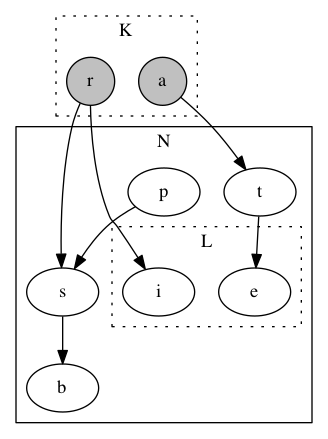
\includegraphics[width=0.35\textwidth]{testGraph2}
\vspace{-0.4cm}
\caption{words in $N$, $L$, and $K$ are related}
\end{figure}
\par In such circumstances, we should deviate from the exact string/phrase matching approach to a \emph{weighted relatedness} approach. \emph{To this end we relate the basic units (words, in this case) found in the system generated outputs to the units in the reference sets}. To be maningful, the semantic relations need to be relativized to an ontology. As the first approximation we use WordNet to find synset based similarity for evaluation but a richer, more knowledge intensive
source like Wikipedia is planned as a future development.
\subsection*{The Equivalence Class}
WordNet~\cite{Miller1990} groups words into sets of synonyms called synsets, provides short definitions and usage examples, and records a number of relations among these synonym sets or their members. WordNet can be seen as a combination of dictionary and thesaurus. Both nouns and verbs are organized into hierarchies, defined by hypernyms or \emph{IS-A} relationship. \emph{The words at the same level represent synset members}. Each set of synonyms has a unique index, representing an equivalence class.   We will test the overlap between two equivalence classes to count a match, along with the exact string/word matching approach.  
\begin{table}[h]
\centering
\resizebox{\columnwidth}{!}{%
\begin{tabular}{c l} 
\toprule
\underline{Words in Abstract:} $K$ & Synset\\
data & \{('datum.n.01'), ('data.n.01')\}\\\midrule
\underline{TextRank Generated Summary:} $L$ & Synset\\
information & \{('information.n.02'), ('information.n.01'), ('information.n.05'), ('data.n.01'), ('information.n.03')\}\\

\bottomrule
\end{tabular}}
\caption{Synset-based Similarity Measure}
\label{keTable}
\end{table}

%We have used the \emph{conceptual path similarity} in our evaluation tool. The path similarity is defined using the \emph{shortest path length in IS-A taxonomy}~\cite{RMBB89} between two word-senses. The score is in the range 0 to 1, except in those cases where  a path cannot be found (will only be true for verbs as there are many distinct verb taxonomies). A score of 1 represents identity i.e. comparing a sense with itself will return 1. Hence, $path\_similarity(w_l, w_k)$ at eq.~\ref{score} depends on the closeness of the two concepts in the taxonomy.  
\par We have applied a \emph{POS-tagger} to fine-tune the synsets for summaries. While evaluating keyphrases, we have considered only words POS-tagged as $nouns$.
%A simple node-counting scheme (path). The relatedness score is inversely proportional to the number of nodes along the shortest path between the synsets. The shortest possible path occurs when the two synsets are the same, in which case the length is 1. Thus, the maximum relatedness value is 1.


\section{Scoring Approach}
For the scientific article set, we combine the  \emph{diamond standard} consisting of author-provided summaries and keywords together with \emph{TextRank} as a test system. For each paper, the TextRank algorithm generates a summary and a set of keywords. The TextRank graph  builds directed edges between the words if they co-occur within a window range and/or they share some common synsets.
\par After generating keyphrases and summaries, we use a modified version of eq.~\ref{eq:imeasure} to score the system. We adapted the WordNet provided \emph{synsets} to detect \emph{similarity} between two synsets of the system output and the diamond standard. 
%\begin{equation}
%\begin{split}
%score(L) = i\hbox{-}measure(N,K,L) \times \\
%                 \sum_{w_l \in L} max \{path\_similarity(w_l, w_k), \forall w_k \in K\}
%\end{split}
%\label{score}
%\end{equation}
The evaluation code considers only one highly trustable  (``diamond standard'') reference per document
contrary to systems like ROUGE or confidence-based Scoring~\cite{DBLP:conf/ecir/HamidHT16}.
\section{Building the Dataset}
We have collected data (conference papers) from several proceedings of $WWW$ and $KDD$ using $CiteSeer^{x}$ digital library. Our choice for WWW and KDD was motivated by the availability of author-assigned keyphrases for each paper. We avoided posters as their internal structure is more complex and contains more figures than texts. Our dataset is composed with a total of 1000 articles. We have used the \emph{pdf2txt} tool in order to convert the original paper to a plain text format. We applied several techniques such as POS-tagger, and an online dictionary to detect/rejoin common words that were split due to the complex pdf structure or column division.  
The dataset is categorized into three sections: 
\begin{itemize}[noitemsep, nolistsep]
\item diamond standard dataset (original paper and it's raw text, body of the paper, abstract, keyphrases)
\item classic textrank generated output (summary, keyphrases, $i\hbox{-}measure$ based statistics)
\item evaluation tool (python source code)
\end{itemize}
 The dataset can be downloaded from \url{https://github.com/abc/dataset_ictir}, free for research purposes.
 \footnote{The original link is distorted due to blind review issue}
\section{Case Study}
In order to explain the usefulness of the evaluation tool, we pick the keyphrase extraction task and a sample document as our case study. We show why/how the evaluation tool is more effective than the absolute scale. 
\begin{table}[h]
\centering
\begin{tabular}{c} 
\toprule
Title: session-juggler secure web login from an untrusted ...\\\midrule
\underline{Author-assigned Keyphrases:} $K$\\
mobile, {\it session}, hijacking, secure, {\it login}, cookies\\\midrule
%\end{tabular}
%\begin{tabular}{c} 
%\toprule
\underline{TextRank Generated Keyphrases:} $L$\\
session, user, site, phone, terminal, juggler, website, logout,\\
browser, web, login, password, bookmarklet, http, untrusted\\
\bottomrule
\end{tabular}
\caption{Diamond Standard \& TextRank Output}
\label{keTable}
\end{table}
\vspace{-.2cm}
\par Table~\ref{keTable} shows that $|K| = 6$, $|L| = 15$, and $|N|$ was counted as $849$. The average-size of intersection, $i$ is $\frac{6 * 15}{849}$, which is $0.016$. And there is $2$ exact match, i.e. $\omega = 2$.
Therefore, $i\hbox{-}measure = \frac{2}{0.016}$, i.e., $18.866$. We can range the size of system output from $0$ to a reasonable point, and find the corresponding $i$ and $\omega$, therefore, draw a performance graph for the system. 
\par It is worth mentioning that several words from the TextRank  output are closely related to the diamond standard: \emph{\{(login, logout), (mobile, phone), (login, password), (secure, untrusted), (mobile, user)\}} and so on. As we also see some TextRank-extracted words in the title, it is clear that these words are closely \emph{related} and \emph{important} for the paper. We should not completely ignore these \emph{words/phrases}. Hence, it is necessary to have a new mechanism for evaluation. Using some domain specific ontology might be a better approach; but for now, we can at-least use the WordNet, which is quite large at size and usable for any domain.  
\section{Conclusion}
%Accurate computer-based evaluation of system-generated summaries (or keyphrases) is far from a being obvious or easy. Most of the shortcomings might come from the simplifications that statistical measures need to assume. 
Accurate evaluation is useful - including for their use in machine learning. Tools like the $i\hbox{-}measure$ introduce some flexibility. Our version of $i\hbox{-}measure$ is tolerant towards length variation and uses some semantic information while calculating the system's performance. Besides WordNet, the tool can be enriched with some domain specific ontologies and paraphrase detection techniques. We believe, it will be a great resource to the research community who are working with information extraction from scientific articles. \\ 
%The dataset is large, automatically cleaned, and usable for both keyphrase extraction and summarization tasks. It comes with a trustable set of reference summary and keyphrases. Any machine learning algorithm can train itself using the dataset. Unsupervised algorithms can also use it to test their performances. 


\chapter{Embedding Knowledge-bases for Evaluation}
Texts are not simply a flat list of sentences; they have a hierarchical structure, one in which certain clauses are more important than others~\cite{Hovy:1998:ATS:1119089.1119121}.

\chapter{Summarization Model focused on Sentiment}
\section*{}
We propose an \emph{unsupervised} model to extract two types of summaries \emph{(positive, and negative)} per document based on 
sentiment polarity. 
Our model builds a \emph{weighted polar digraph} from the text, then  evolves recursively 
until some desired properties converge. 
It can be seen as an enhanced variant of \emph{TextRank} type algorithms working with non-polar text graphs.
Each positive, negative, and objective opinion has some impact on the other if they are semantically related or placed close in the document. 
\par Our experiments cover several interesting scenarios.
In case of a one author news article, we notice a significant overlap between the {\em anti-summary}
 (focusing on negatively polarized sentences) and the the summary.  
For a transcript of a debate or a talk-show, an anti-summary
represents the disagreement of the participants on stated topic(s) 
whereas the summary becomes the collection of positive feedbacks.
In this case, the anti-summary tends to be \emph{disjoint} from the regular summary. 
Overall, our experiments show that our model 
can be used with TextRank to enhance the quality of the extractive summarization process.
\section{Introduction}
 \par A document expresses a writer's opinions along with facts. Usually an article covering several issues will qualify some with positive feedback and some with negative. A high quality summary should reflect the most ``important'' ones amongst them. \emph{Summarization} is thus closely related to \emph{sentiment analysis}. There has been limited work done on the intersection of text summarization and sentiment analysis. Balahur~\cite{conf/paclic/BalahurKSSM09} showed a technique of sentiment based summarization on multiple documents. They used a supervised sentiment classifier to classify the blog sentences into three categories (positive, negative, and objective). 
The positive and the negative sentences are, then fed to the summarizer separately to produce one summary for the positive posts and another one for the negative posts. %Thus, for each blog thread their model produced two summaries. 
The success of their model mostly depends on the performance of the sentiment classifier. Besides, their summarizer does not consider the impact of positive (negative) sentiments while producing the summary of negative (positive) sentiments. It sounds unintuitive to totally separate the sentiment-flows before producing the summaries. Manning \cite{Beineke+al:04a}, in their \emph{sentiment summary} paper used \emph{Rotten Tomatoes} dataset (for training and testing) to extract the most important \emph{paragraph} from the reviewer's article. They aimed at \emph{capturing the key aspects of author's opinion} about the subject (movie). They worked with a \emph{supervised} technique and articles with \emph{single topic}.

\par In this work, we propose an unsupervised, mutually recursive model that can represent text as a graph labeled with polarity annotations.  
Our model builds a graph by collecting words, and their lexical relationships from the document. It handles two properties (\emph{bias} and \emph{rank}) for each of the important words. We consider \emph{sentiment polarity} of words to define the bias. The \emph{lexical definition} and \emph{semantic interactions} of one word to others help defining edges of the text-graph. Thus we build a \emph{weighted directed graph} and apply our model to get the top (positively and negatively ranked) words. Each word in our graph starts with the same \emph{rank}, which eventually converges to some distinct values with the effect of \emph{bias} of its neighbors and \emph{weighted in-links}. Those words then specify the weight of each sentence and grant us a direction to choose important ones. The \emph{bias} of a node gets updated from the \emph{rank} of it's neighbors. The mutual dependency of the graph elements represents the impact of the author's sentiment. Our concept is analogous to {TextRank} algorithm, except -
\begin{small}
\begin{itemize}
\item Our model works for a polar graph whereas TextRank works with non-polar one. 
\item The rank of a node in TextRank gets updated by the connectivity (weighted/ unweighted), whereas the rank in our model gets updated based on the weighted links and bias of its neighbors.
\end{itemize}
\end{small}
\par To the best of our knowledge, our concept of \emph{anti-summary} is new. Hence it was hard to compare the results with a gold standard. We have chosen DUC2004 dataset and basic TextRank algorithm for comparative study. Through our experiments, we have found the following interesting facts -
\begin{small}
\begin{itemize}
\item When the anti-summary and summary are mostly \emph{disjoint}, the document is a collection of different sentiments on stated topics. It can be a transcript from some debate, political talk, controversial news, etc.
\item When the anti-summary \emph{overlaps} at a noticeable amount with the summary, the document is a news article stated from a neutral point of view.
\item By blending anti-summary with TextRank generated one, we show another way of producing \emph{opinion-oriented} summary which not only contains the flow of negative sentiment but also includes facts (or some positive sentiment).
\end{itemize}
\end{small}
\section{Background Study}
\par Automated text summarization dates back to the end of fifties~\cite{Luhn:1958:ACL:1662353.1662360}. A summarizer deals with the several challenges. To extract important information from a huge quantity of data while maintaining quality are two of them. A summarizer should be able to understand, interpret, abstract, and generate a new document.
Majority of the works focus on \emph{``summarization by text-span extraction''} which transforms the summarization task to a simpler one: ranking sentences from the original document according to their salience or their likelihood of being part of a summary~\cite{Goldstein:1999:STD:312624.312665}.
\par Early research on extractive summarization was based on simple heuristic features of the sentences such as their position in the text, frequency of words they contain etc. More advanced techniques also consider
the relation between sentences or the discourse structure by using synonyms of the words or anaphora resolution. 
To improve generic machine generated summaries, some researchers~\cite{Goldstein:1999:STD:312624.312665} converted some hand-written summaries (collected from the Reuters and the LosAngeles Times) to their corresponding extracted ones.  Based on their experiments, they stated that \emph{summary length is independent of document length.} Though Hovy and Lin \cite{Hovy:1998:ATS:1119089.1119121} stated earlier, ``A summary is a text that is produced out of one or more texts, that contains the same information of the original text, and that is {\em no longer than half} of the original text.'' For our experiments, we will generate summaries with at-most top ten sentences per document.
\par Graph based ranking algorithms have recently gained popularity in various natural language processing applications; specially in generating {\em extractive summaries}, selecting keywords, forming word clusters for sense disambiguation, and so on. They are essentially a way of deciding the importance of a vertex within a graph, based on global information recursively drawn from the entire graph~\cite{Mihalcea04TextRank}. The basic idea is of ``voting'' or ``recommendation''. When one vertex links to another one, it is basically casting a vote for the other vertex. The importance of the vertex casting the vote determines how important the vote itself is.  Hence the score (usually called {\em ``rank''}) associated with a vertex is determined by the votes cast for it, and the score of the vertices casting these votes. TextRank works well because it does not rely on the local context of a text unit and requires no training corpus, which makes it easily adaptable to other languages or domains. Erkan and Radev \cite{Erkan:2004:LGL:1622487.1622501} in \emph{LexRank} (another graph based ranking algorithm to produce multi-document summary) used \emph{the centrality of each sentence in a cluster} to assess the importance of each sentence. To measure the similarity between two sentences, they used cosine similarity matrix (based on word overlap and {\em idf (inverse document frequency)} weighting). Being inspired by the success of textrank models, we had the idea to apply a {\em polar textrank} model in order to extract sentences from {\em negative (positive)} point of view.
\par It is important that we consider each sentiment of the author while producing the summary. In our work, we adopt a graph based ranking model which originally was proposed for {\em trust-based (social, peer-to-peer) networks}~\cite{Mishra:2011:FBP:1963405.1963485}. It intends to measure the prestige (rank) of nodes (participants in the event) present in the graph. Their hypothesis, {\em ``the node which is prone to trust (mistrust) all its neighbors is less reliable than the node who provides unpredictable judgments,''} works also for producing summaries. Each node (word) has weighted (positive/negative/neutral) directed links to its neighbor nodes (other words, possibly collected from the same sentence or nearby sentences). The more weight it provides to its neighbors the more importance (either positive or negative) it indicates. The impact is higher when a node behaves differently (a positive biased node has a negative weighted outline or vice versa) towards its neighbors. 

\section{Anti-Summary}
We propose an extractive summarization technique which produces anti-summaries as well as summaries for each document. We would discuss what anti-summary is and why it is important. Sentences with upstream knowledge
are the candidates of anti-summary. A sentence does not have to contain words like \emph{\{no, neither, never, not, ever, bother, yet, \dots\}}, to be the part of the anti-summary. 
\par We can start with a generic example:  A document is about topic $A$. It is comparing the qualities of $A$ with related topics $B$, $C$, and $D$. Suppose, topic $B$ is mostly receiving negative opinions in that document. Then a summary of the document should include positive feedbacks on $A$ and the anti-summary should be more about the properties of $B$.
\vspace{-.25in}
\begin{figure}
\begin{center}
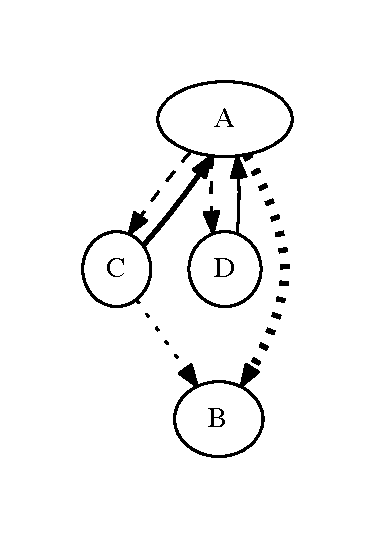
\includegraphics[width = 0.29\textwidth, scale = .22, angle = 90]{testGraph.pdf}
\vspace{-.45 in}
\caption{A text-graph describing several topics}
\end{center}
\end{figure}
\vspace{-.3 in}
\par Anti-summaries are as important as summaries.  They help us find relative materials on a specific topic. For example, from a news article, without any supervised topic detection, anti-summaries can indicate which parts of it represent negative/ suppressed opinion. In a scientific article, anti-summaries tell how system $A$ is different/ better/ worse than system $B$ where as summaries might only tell us the usefulness of system $A$.  
\par Interestingly enough, some summary sentences are also present in anti-summary of the document. This means, anti-summaries are not exactly opposite to summaries, it is the reverse stream of the main news. Anti-summaries can help a search engine build comparative database. It is intuitive that two documents are related if there is a significant match between one's summaries and the other's anti-summaries.

\section{Sentiment Analysis: Covering Minimal Issues}

\emph{Sentiment Analysis} has important aspect on fields which are affected by people's opinions, e.g., politics, economics, social science, management science and so on. It plays a vital role in every aspect of NLP; for example, co-reference resolution, negation handling, word sense disambiguation etc. \emph{Sentiment words} are instrumental to sentiment analysis~\cite{doi:10.2200/S00416ED1V01Y201204HLT016}. Words like \emph{good, wonderful, amazing} convey positive connotation whereas \emph{bad, poor, terrible} are used to flow negative sense. As an exception, some adjectives and adverbs (e.g. \emph{super, highly}) are not oriented clearly to either one of the poles (positive, negative). A list of sentiment words are called \emph{sentiment lexicon}. A sentiment lexicon is necessary but not sufficient for sentiment analysis.
\par A positive or negative sentiment word may have opposite orientations in different application domains, e.g., \emph{``The vacuum cleaner sucks!''} vs. \emph{``The camera sucks.''} Sentiment words may be used objectively rather subjectively in some sentences, e.g., \emph{``If I can find a good camera, I can buy that.''} Sarcastic sentences are trickier to handle, as well as sentences having no sentiment word but with a sentiment expressed.
\par Based on the level of granularities (document level, sentence level, entity and aspect level) we choose the \emph{entity level} analysis of sentiments. For example, the sentence, ``The iPhone's call quality is good, but its battery life is short,'' evaluates two aspects: \emph{call quality} and \emph{battery life}. The two opinion targets for this sentence, \emph{call quality} has positive sentiment and \emph{battery life} has negative.
\par Our model is unsupervised, and we decided not to use statistical database to calculate the sentiment polarity for sentences/ paragraphs/ document. Hence we have used only a {\em sentiment lexicon} to get the usual sentiment polarity at word level.

\section{The Polarity based TextRank Model} 
Jon Kleinberg's \emph{HITS} or Google's \emph{PageRank} are two most popular 
graph based ranking algorithms, successfully used for analyzing the link-structure of world wide web, citation graph, and social networks. A similar line of thinking is applied to semantic graphs from natural language documents, resulting in a graph based ranking model, TextRank~\cite{Mihalcea04TextRank}. The underlying hypothesis of TextRank is that in a cohesive text fragment, related text units tend to form a web of connections that approximates the model humans build about a given context in the process of discourse understanding. TextRank, with different forms (weighted, unweighted, directed, undirected) of graphs, was applied successfully for different applications, specifically for text summarization~\cite{Mihalcea04graph-basedranking}. Based on the results so far, it performed well for summarizing general text documents. There are documents which present arguments, debates, competitive results and they are subjective reflections of the author(s). The limitation of TextRank (and other similar models) is that it does not handle 
negative recommendations different from positive ones. In this work, we present a different model~\cite{Mishra:2011:FBP:1963405.1963485} that can be adopted to have the impact of sentiments on the summary. 
 \subsection{Trust Based Network}
 \par A network based on trust (e.g. facebook, youtube, twitter, blogs) is quite different from other networks; in each case, reputation of a peer as well as types of opinion (trust, mistrust, neutral) matters. An explicit link in a \emph{trust-based} network indicates that two nodes are close (connected), but the link may show either \emph{trust} or \emph{mistrust}. A \emph{neutral} opinion in a trust based network is different from \emph{no-connection}. TextRank gives higher ranks with better connectivity. The situation changes dramatically in trust based networks as a highly disliked node may also be well connected. To take care of this situation, authors~\cite{Mishra:2011:FBP:1963405.1963485} correlated two attributes for each node: \emph{Bias} and \emph{Prestige}. 
\subsubsection{Bias \& Prestige}
\par The bias of a node is the propensity to trust/ mistrust other nodes. The prestige of a node is the ultimate rank (importance) of it in compared to other nodes.
Formally, let $G=(V,E)$ be a graph, where an edge $e_{ij}\in E$ (directed from node $i$ to node $j$) has weight $w_{ij} \in [-1, 1]$. $d^o(i)$ and $d^i(i)$ correspondingly denote the set of outgoing links from and incoming links to node $i$. Bias reflects the expected weight of an outgoing edge. Using bias, the inclination of a node towards trusting/ mistrusting is measured. The bias of node $i$ can be determined by 
\begin{small}
\begin{equation} 
\label{biasEq}
bias(i) = \frac{1}{2|d^o(i)|}\sum_{j \in d^o(i)} (w_{ij} - rank(j))
\end{equation}
\end{small} 
Prestige (rank) reflects the expected weight of an in-link from an un-biased node. Intuitively, when a highly biased node (either positive or negative)  gives a rating, such score should be given less importance. When a node has a positive (negative) bias and has an edge with a negative (positive) weight, that opinion should weigh significantly. Hence, the prestige (rank) of node $j$ could be determined as
\begin{small}
\begin{equation}
\label{rankEq}
rank(j) = \frac{1}{|d^i(j)|}\sum_{k \in d^i(j)}(w_{kj}(1 - X_{kj}))
\end{equation}\end{small}
where the auxiliary variable $X_{kj}$ determines the change on weight $w_{kj}$ based on the bias of node $k$.
\begin{small}
\begin{equation}
\label{auxEq}
X_{kj}=\begin{cases}
0  & \textit{if ($bias(k) \times w_{kj}) \le 0$},\\
|bias(k)|  & \textit{otherwise}.
\end{cases}
\end{equation}
\end{small}
After each iteration of \ref{biasEq} and \ref{rankEq}, edge weight $w_{kj}$ is scaled from the old weight as follows:
\begin{small}
\begin{equation}
\label{weiEq}
w_{kj}^{new} = w_{kj}^{old}(1 - X_{kj}) 
\end{equation}
\end{small}
\section{Text as Graph}
\label{textAsGraph}
In order to apply the graph based ranking algorithms, we convert the text document into a graph.
We extract words (except stop-words) from each sentence and represent them as \emph{nodes} of our graph. 
Each pair of related words ({\em lexically} or {\em semantically}) forms the \emph{edges}.
We use \emph{SentiWordNet} (a publicly available lexical resource for opinion mining) to determine the sentiment polarity of each node (signature word). SentiWordNet~\cite{Esuli06sentiwordnet:a}
assigns to each synset of \emph{WordNet}~\cite{Miller95wordnet:a} three sentiment scores: positivity, negativity, and objectivity. 
We choose the highest (most common) sentiment polarity of a word as the \emph{bias}. Edge weights are determined by the total outgoing edges from the node. If there is a \{not, no, though, but,\dots\} present between $word_a$ and $word_b$, the edge weight ($w_{ab}$) receives the opposite sign of $bias_a$. Our algorithm performs the following steps:- 
\begin{itemize}
\item Phase I: Build the Text-Graph
\begin{small}
\begin{itemize}
\item Collect signature words; use them as \emph{nodes} for the graph.  Use their sentiment polarity as \emph{bias}.
\item Add edges between nodes (words) that reside in the same sentence (within a chosen window size).
\item Assign edge-weights ($w_{ab}$) based on the total outgoing edges from each source node ($word_a$).
\item Update/ add edge-weights ($w_{ab}$) if they are semantically related (e.g., use a matching function on their definition/synonym list).
\item Assign a random value as \emph{rank} to all the nodes of the graph (initially all nodes are on the same level).
\end{itemize}\end{small}
\item Phase II: Apply Ranking Model
\begin{small}
\begin{itemize}
\item  Apply formula [\ref{biasEq},\ref{rankEq},\ref{auxEq},\ref{weiEq}] over the graph until the $rank$ value converges.
\end{itemize}
\end{small}
\item Phase III: Find Ranked Word Vectors, \& Extract Sentences
\begin{small}
\begin{itemize}
\item Create a positive word vector, $W^{pos}$ of {\em keywords} by selecting all positively ranked words.
\item Create a negative word vector, $W^{neg}$ of {\em keywords} by selecting all negatively ranked words.
\item Use $W^{pos}$ and $W^{neg}$ to determine the weight and orientation of the sentences.
\item Group top $k$ (can be determined by the user) negatively (positively) oriented sentences as {\em anti-summary (summary)}.
\end{itemize}
\end{small}
\end{itemize}
\vspace{-.1in}
\par The following subsections will discuss our process in detail. To demonstrate several intermediate  outcomes of our 
process, we will use a sample article: \url{http://students.cse.unt.edu/~fh0054/SummaryAnti/Kennedy1961/kennedyPart1.txt}, 
which is a small fragment (only 77 sentences are considered) of President Kennedy's speech in 1961.
\vspace{-.1in}
\subsection{Signature Words}
Using a standard {\em parts of speech tagger}, we extract words that are labeled as either one from the set: {\em \{noun, verb, adjective, adverb\}}. These are our {\em signature words}. We also collect their {\em definition} and {\em sentiment polarity} for the next phase.
Table~\ref{wordx},~\ref{wordy} show the intermediate data generated from example $01$. 
\par {\em Example 01: The first and basic task confronting this nation this year was to turn recession into recovery.}  
\subsection{Define Nodes \& Edges: From a single sentence}
Let, $x$ and $y$ are two words residing in the same sentence, and $|position_x - position_y| < window$ $size$. We create distinct nodes (if not already exist) for $x$ and $y$, and define their relations (edges) by either of the rules:
\begin{small}
\begin{itemize}%[noitemsep,nolistsep]
\item If $parts\_of\_speech(x) = \{verb\}$, add $edge(x,y)$. 
\item If $parts\_of\_speech(x) \cup parts\_of\_speech(y) \\ \subset \{noun, adjective,adverb\}$, then 
 add $edge(x,y)$ and $edge(y,x)$.
\item Finally, we add edge-weight, $w_{xy} = sign(bias(x))\times\frac{1}{|E|} $ to all the existing edges.
\end{itemize}\end{small}
\subsection{Connect Sentences through Words: Add more Edges/ Update Weights }
Let $x$ and $y$ are two different words from two different sentences (or from the same sentence,
$|position_x - position_y| \ge window$ $size$). We use their \emph{definition} (available in WordNet) to determine $similarity$ between them. 
If $def(x)$ stands for $definition$ of $x$, 
\begin{small}
\begin{equation}
similarity(x, y) = \frac{def(x) \cap def(y)}{def(x) \cup def(y)}
\end{equation}
\end{small}
\vspace{-.1in}
We add/ update edge-weight $w_{xy}$ and $w_{yx}$ using the following manners:
\begin{small}
\begin{itemize}%[noitemsep,nolistsep] 
\item We do not update the graph if the $similarity(x,y)$ is $zero$.
\item For an \emph{existing} edge between $x$ and $y$, we adjust $w_{xy}$ as $w_{xy} + similarity(x,y)\times sign(bias(x))$. 
\item For a \emph{no edge} between $x$ and $y$, we add two new edges ($edge(x,y)$ and $edge(y,x)$) where $similarity(x,y)$ acts as the weight for the new edges. 
\end{itemize}
\begin{figure}
\CenterFloatBoxes
\begin{floatrow}
\killfloatstyle
\capbtabbox{
\resizebox{.5\textwidth}{!}{
\begin{tabular}{ l l r p{5cm}}
\toprule
Word & PoS & Polarity & Definition \\
\midrule
first & adj & $0.0$ & preceding all others in time or space or degree\\
confront & v & $-0.5$ & oppose, as in hostility or a competition\\ 
nation & n & $0.0$ & a politically organized body of people under a single government\\
year & n & $0.0$ & a period of time containing 365 (or 366) days\\
turn & v & $0.0$ & change orientation or direction, also in the abstract sense\\
recession & n & $0.0$ &the state of the economy declines; a widespread decline in the GDP and employment and trade lasting from six months to a year\\
recovery & n & $0.0$ &  return to an original state\\
\bottomrule
\end{tabular}
}}{\caption{Words \& Their Entities}\label{wordx}
}
\killfloatstyle
\capbtabbox{
\resizebox{.5\textwidth}{!}{
\begin{tabular}{ l p{5cm}  r}
\toprule
Word & Definition & Similarity\\
\midrule
\midrule
recession&the state of the economy declines; a widespread decline in the GDP and employment and trade lasting from six months to a year &\\
recovery& return to an original state &0.035714\\
\midrule
security &the state of being free from danger or injury&\\
progress & gradual improvement or growth or development& 0.0\\
\midrule
recovery & return to an original state\\
security &the state of being free from danger or injury&  0.071428\\
\bottomrule
\end{tabular}}}{ \caption{Degree of Similarity}\label{wordy}}
\end{floatrow}
\end{figure}
\end{small}
This phase helps relate semantically closer words in the document. 
\par To demonstrate how the graph is formed, we randomly picked two sentences from the stated article:
{\em `Our security and progress cannot be cheaply purchased; and their price must be found in what we all forego as well as what we all must pay'} and {\em `The first and basic task confronting this nation this year was to turn recession into recovery'}.
The sentence graph with only these two sentences (with $window$ $size = 4$) is shown in figure~\ref{sfig}. 
\begin{figure}
\CenterFloatBoxes
\begin{floatrow}
\ffigbox{
\resizebox{.5\textwidth}{!}{
 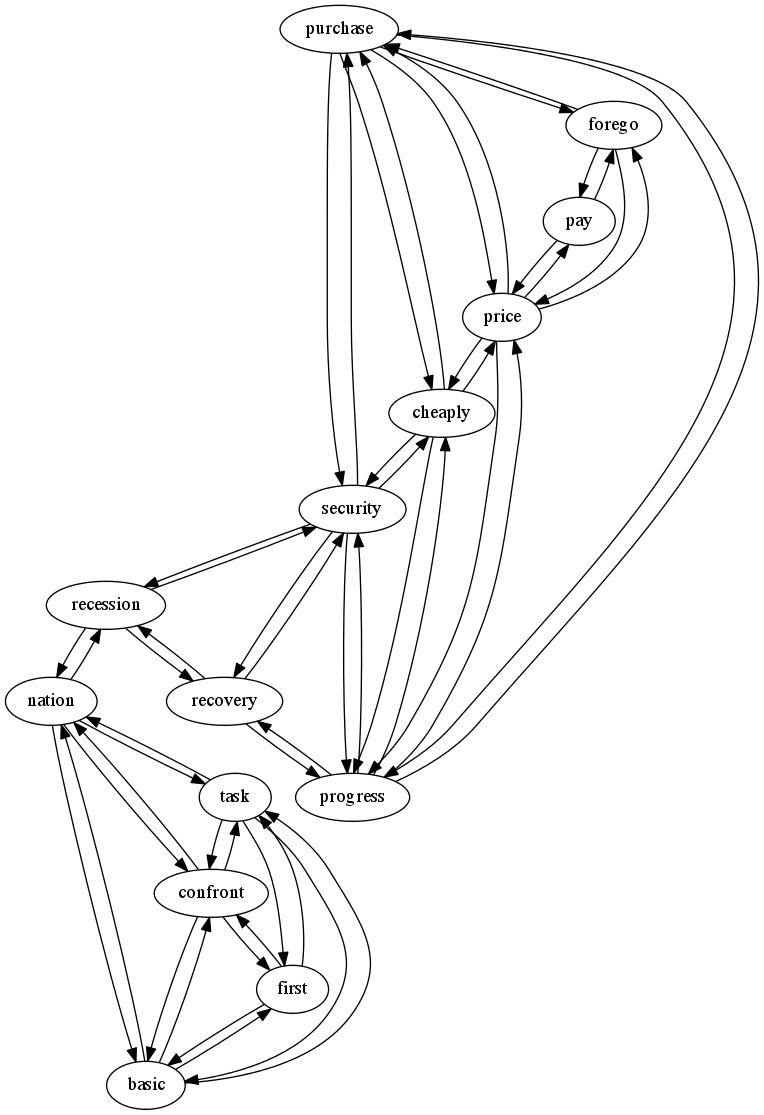
\includegraphics[scale=0.25]{gx3.png}
}}
{\caption{Sentence Graph}\label{sfig}
}
\killfloatstyle
\capbtabbox{
\begin{tabular}{l r l}
\toprule
keyword & Rank&\\
\midrule
initiate & 1.50503400134e-07&\multirow{10}{20pt}{positively ranked}\\
wisely & 2.37049201066e-19\\
cheaply & 2.03124423939e-19\\
thailand &1.52162637924e-28\\
believe & 2.53398571394e-38\\
crucial & 1.14205226912e-40\\
forego & 7.26752110553e-46\\
mind & 3.3034186848e-46\\
handicap & 1.89292202562e-57\\
progress & 1.18505270306e-62\\
\midrule
cambodia & -0.0210985300569 &\multirow{10}{50pt}{negatively ranked}\\
recovery & -0.126687287356 \\
recession & -0.0376108282812 \\
unwilling & -7.70602663247e-05\\ 
congress & -0.064049452945 \\
cooperate & -0.285579113282\\
building & -0.0387114701238\\
havana & -0.0128506602917\\ 
frontier & -0.0182778316133\\ 
compete & -0.075853425471\\
\bottomrule
\end{tabular}
%\end{centering}
%\end{table}
}
{\caption{A subset of Keywords}\label{finalKeys}
}
\end{floatrow}
\end{figure}
We notice that word pairs {\em \{(security, recession), (security, recovery), (progress, recovery)\}}, for example, are connected to each other through the {\em similarity} relationship.
\subsection{Keyword Extraction}
\par Once the graph is built, we add a real value (can be chosen randomly) 
to every node as it's $rank$. This way, there is no discrimination
beforehand. Then we apply set of equations [\ref{biasEq},\ref{rankEq},\ref{auxEq},\ref{weiEq}] several times (until the
rank value converges) over the graph. For real time output, one can control
the repetition using a threshold. 
Table~\ref{finalKeys} shows a handful of positively ranked and negatively ranked keywords (out of $568$ total words) from the same article. 
\subsection{Sentence Extraction}
Our top (positive, and negative) ranked keywords define the weights of the sentences. Let $W^{pos}$ ($W^{neg}$) be the list of words achieving positive (negative) rank values. Let $W^{pos}$ is a list of size $m$ and $W^{neg}$ is a list of size $n$.% where $m + n = $ total number of nodes. 
Weight of a sentence, $s_j$ is:
%We define $W^{pos} = \{ rank(v_i) \mid v_i \in V^{pos}, 1 \le i \le m\}$, and $W^{neg} = \{ rank(v_i) \mid v_i \in V^{neg}, 1 \le i \le n\}$.
\begin{subequations}
\begin{align}
weight(s_j^{neg}) = (\sum_{v_i \in W^{neg} \wedge v_i \in s_j}|rank({v_i})|) / (n \times |s_j|),\\
weight(s_j^{pos}) = (\sum_{v_i \in W^{pos} \wedge v_i \in s_j }rank({v_i})) / (m \times |s_j|),
\end{align}
\end{subequations}
Now each sentence has two weights associated with it; $weight(s_j^{pos})$ corresponds its weight on positively ranked words whereas 
$weight(s_j^{neg})$ corresponds its weight on negatively ranked words. Thus $S^{neg}$ ($S^{pos}$) forms a weight vector of sentences on negatively (positively) ranked ones.
One can select top $k$ many sentences based on $S^{neg}$ as the {\em anti-summary}. The similar line of thinking goes for generating regular summaries. To avoid promoting longer sentences, we are using length of the sentence as the \emph{normalization factor}.
%and divide the $weight(s_j)$ with the length of sentence $s_j$. 
\begin{table}[h]
\begin{centering}
\resizebox{.9\textwidth}{!}{
\begin{tabular}{p{9cm} r}
\toprule
sentence & weight\\
\midrule
Our security and progress cannot be cheaply purchased; and their price must be found in what we all forego as well as what we all must pay.  &$1.98797587956e-14$\\
\midrule
The first and basic task confronting this nation this year was to turn recession into recovery. & $-0.00117486599011$\\
\bottomrule
\end{tabular}}
\caption{Sample of top sentences}
\label{table:finalSents}
\end{centering}
\end{table}
 \vspace{-0.2in}
Table~\ref{table:finalSents} shows two top sentences(the first one is the $2^{nd}$ top positively ranked and the second one is $5^{th}$ top negatively ranked). The original file can be found at: \url{http://students.cse.unt.edu/~fh0054/SummaryAnti/Kennedy1961/kennedyPart1SA.txt}.%{``Summary of Kennedy's Speech''(link)}.
\par Our model uses  a mutually recursive relation on {\em bias} and {\em rank} calculation. It incrementally updates the {\em edge-weights} as well. Hence, it helps get the final ranks (polarity and weights) of words on global context. Since a textrank model does not rely on the local context of a text unit, and requires no training corpus, it is easily adaptable to other languages or domains.

\section{Evaluation}
We used TextRank (extracted) and Human (abstract) summaries from DUC 2004 (task 1) as the baseline. TextRank is unsupervised and it does not handle sentiment polarity. Hence, we started with hypothesis~\ref{h1}.
\begin{hyp}
\label{h1}
 polarity based summaries and anti-summaries should almost equally intersect with TextRank generated ones.
 \end{hyp} 
In order to verify the hypothesis, we calculated average number of sentence intersection between each pair of the three summaries (our model generated anti-summary($N$), summary($P$) and textrank summary($T$)). Then we plotted them against the probability of intersection of two random generated summary. Table~\ref{myT} explains the operations. The test cases are named as -
\begin{itemize}
\item case a: an average size of  ($P \cap T$),  
\item case b: an average size of  ($N \cap T$),  
\item case c: an average size of  ($P \cap N$),  
\item case d: an average size of ($S_1 \cap S_2$), with any two randomly selected set $S_1$ and $S_2$ of the same size as $P$, $N$ and $T$.
\end{itemize}
(Summaries of these set of articles are stored in link: \url{http://students.cse.unt.edu/~fh0054/cicling2015/}).
\begin{table}[ht]
\begin{centering}
\resizebox{.9\textwidth}{!}{
\begin{tabular}{ p{7mm} L{10 mm} R{13mm} R{13mm} R{13mm} R{13mm} R{13mm} R{13mm} R{13mm}}
\toprule
Test Set&Total Files&no of sentences per file($n$)&$avg(n)$&summary size($k$ sentences) & $avg(k)$&case $a$& case $b$ &case $c$\\
\midrule
1&163&$n > 30$&$48$&$10$&$10.00$&1.75&3.18&1.43\\
\midrule
2&337&$n \le 30$&$16.5$&$n/3$&$5.10$&1.63&1.88&1.08\\
%\cline{5-9}
&&&&$n/2$&$8.05$&4.21&4.73&3.386\\
\midrule
3&410&$n \le 40$&$20.02$&$n/3$&$6.34$&2.626&2.304&1.44\\
%\cline{5-9}
&&&&$n/2$&$9.775$&5.826&5.613&4.256\\
\bottomrule
\end{tabular}
\caption{summary \& their average size of intersection\label{myT}}}
\end{centering}
\end{table}
 \vspace{-0.3in}
Quite interestingly, for shorter articles, \emph{case a} and \emph{case b} showed similar (and better) performance than \emph{case c} and \emph{case d} [table~\ref{myT}, \& figure~\ref{random}]. It also supports hypothesis~\ref{h1}.
For larger articles, \emph{case b} was the winner. The following section gives the mathematical background for case $d$.
\begin{figure}[ht]
	\centering
	\begin{tikzpicture}	
	                \begin{groupplot}[group style={group name=my plots,group size= 3 by 1,vertical sep= 0.4 cm, horizontal sep = .4 cm },height=6cm,width=5.1cm]
	                \nextgroupplot[title={Test Set $1$},ylabel={$avg(n,k)$}, xlabel={summary size($k$)},legend style={fill=none, xshift = -1.5cm}]
          \addplot[
		scatter/classes={
			a={mark=oplus},%
			b={mark=square},%
			c={mark=triangle}%
		},
		scatter,only marks,
		scatter src=explicit symbolic]
	              table[x=x,y=y,meta=label]
			{points48.dat};
	
          
          	\addplot [black] coordinates{
			(5,   0.52083)
			(6,   0.75)
			(7, 1.02083)
			(8, 1.33333)
			(9, 1.6875)
			(10, 2.083333)
			(11, 2.52)
				};
		 \legend{case a, case b, case c, case d}		
		\addplot [dotted] coordinates {
		         (10,0)
                 (10,1)
                 (10,2)
                 (10,4)
                 (10,5)     
               } node[pos=0.8,pin=90:{\color{black}$k$}] {};	
               

   \nextgroupplot[title={Test Set $2$},legend style={fill=none, xshift = -2.5cm}]  
	    \addplot[
		% clickable coords={\thisrow{label}}, 
		scatter/classes={
			a={mark=oplus},%
			b={mark=square},%
			c={mark=triangle}%
		},
		scatter,only marks,
		scatter src=explicit symbolic]
	              table[x=x,y=y,meta=label]
			{points.dat};
	
	
		\addplot [smooth] coordinates {
			(2, 0.2)
			(3, 0.52)
			(4, 0.94)
			(5, 1.47)
			(6, 2.11)
			(7, 2.88)
			(8,3.76)
			(9,4.73)
			};
            \addplot [dotted] coordinates {
		      (8.05,0)
                 (8.05,1)
                 (8.05,2)
                 (8.05,4)
                 (8.05,5)     
               } node[pos=0.8,pin=90:{\color{black}$k_2$}] {};	
               
            \addplot [dotted] coordinates {
		      (5.10,0)
                 (5.10,1)
                 (5.10,2)
                 (5.10,4)
                 (5.10,5)
                 
               } node[pos=0.4,pin=90:{\color{black}$k_1$}] {};	
               %\legend{case a, case b, case c, case d}
               \nextgroupplot[title={Test Set $3$},legend style={fill=none, xshift = -2.5cm}]  
	    \addplot[
		% clickable coords={\thisrow{label}}, 
		scatter/classes={
			a={mark=oplus},%
			b={mark=square},%
			c={mark=triangle}%
		},
		scatter,only marks,
		scatter src=explicit symbolic]
	              table[x=x,y=y,meta=label]
			{points20.dat};
	
		\addplot [smooth] coordinates {
			(3, 0.45)
			(4, 0.8)
			(5, 1.25)
			(6, 1.8)
			(7, 2.45)
			(8,3.24)
			(9,4.05)
			(10,5)
			};
            \addplot [dotted] coordinates {
		       (9.775,0)
                 (9.775,1)
                 (9.775,2)
                 (9.775,4)
                 (9.775,5)     
                 (9.775,6)     
               } node[pos=0.2,pin=90:{\color{black}$k_2$}] {};	
               
            \addplot [dotted] coordinates {
		       (6.34,0)
                 (6.34,1)
                 (6.34,2)
                 (6.34,4)
                 (6.34,5)
                 
               } node[pos=0.4,pin=90:{\color{black}$k_1$}] {};	
               %\legend{case a, case b, case c, case d}

    	\end{groupplot}
	\end{tikzpicture}
	\caption{average of sentence intersection based on equation ~\ref{binomial}}
	\label{random}
\end{figure}

\subsection{Baseline: \emph{Intersection} of two models vs. the \emph{Random} possibility}
The average size of an intersection($avg$) of subsets with $k$ elements taken from a set with $n$ elements can be determined by eq. ~\ref{binomial}.
\begin{small}
\begin{equation}
\label{binomial}
avg(n,k) = {{\sum_{i=0}^k i \binom{k}{i}\binom{n-k}{k-i}}
\over {\sum_{i=0}^k  \binom{k}{i}\binom{n-k}{k-i}}}
\end{equation}
\end{small}
For two summaries of different sizes $k$ and $l$ this generalizes to:
\begin{small}
\begin{equation}
\label{binomialLK}
avg(n,k,l) = {{\sum_{i=0}^k i \binom{k}{i}\binom{n-k}{l-i}} \over
{\sum_{i=0}^k \binom{k}{i}\binom{n-k}{l-i}}}
\end{equation}
\end{small}
These formulas are justified as follows:
Fix one of the subsets as $X={0,1,\dots,k-1}$.
Then an intersection of size $i$ is computed by taking a subset of
$X$ of size $i$ (there are ($b=\binom{k}{i}$) such sets ). We have $j= l-i$
elements in $X$ that will be selected among the $b'$ subsets of size $j$
of the remaining $n-k$ elements in the complement of $X$ counted as
$b'=\binom{n-k}{l-i}$.
So the numerator of the fraction, will be obtained by summing up for $i=0$ to $k-1$
the product of $i$ with the number of subsets $b$ and 
and the number of subsets $b'$, counting the total length of the subsets. The denominator of the fraction 
will count the total number of these subsets and the result of their division will give the average size of the intersections. 

Knowing the average sizes of the overlap of two summaries of size $k$ or sizes $k$ and $l$ when they are different (seen as sets of words), tells us whether our model-generated summaries, and anti-summaries have a better rate of intersecting with each other (and textrank) than {\em random summaries} would. 

\subsection{Does $(P \cap N)$ indicate something interesting?}
\par In each case, $(P \cap N)$ is minimal (fig. \ref{random}) which indicates that our model is successfully splitting the two flow of sentiments from documents. This raises a set of questions, e.g., 
\begin{small}
\begin{itemize}[noitemsep,nolistsep]
\item when $(N \cap T) \gg  (P \cap T)$, should we label the article as a $negatively$ biased one?% irrespective of topics?   
\item when $(P \cap T) \gg (N \cap T)$,  should we label the article as a $positively$ biased one?% irrespective of topics? 
\item when $(P\cap N) \gg (P \cap T)$ and $(P\cap N) \gg (N \cap T)$, is it a news/article stated from a $neutral$ point of view? 
\end{itemize}
\end{small}
We tried to answer these questions based on experimental results. We might need voluntary human judges
to label the articles based on the the extractive summaries and compare our \emph{summary based guesses}. We leave this phase as a future direction. Interested reader can get our result from the following link:
\url{http://students.cse.unt.edu/~fh0054/cicling2015/summaryHalf/fileType.txt}
\subsection{How much \emph{relevant information} is retrieved?}
We needed to know whether our model is gathering some relevant sentences or not. We use abstractive summaries (provided with DUC2004 dataset) and TextRank extracted ones as base results; then use the \emph{recall} measure to estimate the ratio of number of relevant information retrieved. 
\subsubsection{Recall \& Precision}
Recall ($R$) is the ratio of \emph{number of relevant information received to the total number of relevant information in the system}. If $D$ is the original document, $A$ is the anti-summary, and $S$ is the standard summary, then the recall($R$) value can be calculated from eq. ~\ref{eA1}.
 \vspace{-0.1in}
\begin{center}  
 \begin{minipage}{0.4\textwidth}
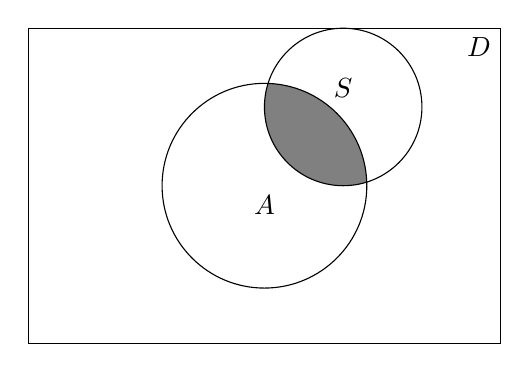
\begin{tikzpicture}
        \draw [anchor = south] \Urectangle node[ below left]{$D$};
       \begin{scope} % start of clip scope
              \clip \firstcircle;
              \fill[gray] \secondcircle;
        \end{scope}
       
        \draw [even odd rule]\firstcircle node[below] {$A$};
         \draw \secondcircle node [above] {$S$};
   \end{tikzpicture}
\end{minipage}%%% to prevent a space
\begin{minipage}{0.4\textwidth}
\begin{equation}
\label{eA1}
R =  \frac{A \cap S}{S}
\end{equation}
\begin{equation}\label{eA2}
P =  \frac{A \cap S}{A}
\end{equation}
\end{minipage}
\end{center}
 \vspace{-0.1in}
\par Another well-known measure is \emph{Precision ($P$)} which is the ratio of {number of relevant records retrieved} to the total number (relevant and irrelevant) of records retrieved (eq. ~\ref{eA2}). 
As our test dataset had different file sizes, we can tune the anti-summary length as we want, and we cannot firmly state that $A \setminus (A\cap S)$ is irrelevant; we believe, interpretation of $R$ is more relevant than $P$, in our case.
\begin{small}
\begin{table}[ht]
\begin{centering}
\resizebox{.99\textwidth}{!}{
\caption{Avg. Recall of P, N, T w.r.t. Human Summary\label{myR}}}
\begin{tabular}{L{7mm}  L{10 mm}  L{13mm}  L{13mm}  R{13mm} R{13mm} R{13mm}}
\toprule
Test Set&Total Files&no of sentences per file($n$)&summary size($k$ sentences) & recall(P) = $\frac{P\cap H}{H}$ & recall(N) = $\frac{N\cap H}{H}$ &recall(T) = $\frac{T\cap H}{H}$\\
\midrule
1&163&$n > 30$&$10$&\maxf{$.469}$&$.397$&$.447$\\
\midrule
2&337&$n \le 30$&$n/3$&$.408$&$\maxf{.458}$&$.457$\\
%\cline{4-7}
&&&$n/2$&$.545$&\maxf{$.596}$&$.583$\\
\midrule
3&410&$n \le 40$&$n/3$&$.449$&$.436$&$.531$\\
%\cline{4-7}
&&&$n/2$&$.588$&$.582$&$.607$\\
\bottomrule
\end{tabular}
\end{centering}
\end{table}
\end{small}
\par Table~\ref{myR} shows the average recall value on the our model generated summary($P$), anti-summary($N$), and textrank($T$) summary with respect to human ($H$) summary. We have used \emph{uni-gram word matching} for computing recall rate. 
%\emph{N-gram},(for example $N ={ 2, 3, \dots}$ ) provides almost the same recall rates.
This result gives us an idea that -
\begin{hyp} 
\label{h2}
Anti-summary can help extending TextRank summary in order to produce sentiment oriented summary.
\end{hyp}

\subsection{Evaluation through examples: ($P\cap N$) is minimal}
\par The next block is a summary and an anti-summary produced by our system, for the data file: \url{http://students.cse.unt.edu/~fh0054/SummaryAnti/googleCase.txt}.
This example shows a clear distinction between the summary and the anti-summary sentences. The {\em summary} sentences represent the view of \emph{European Union and other Companie}s questioning Googles privacy policy. On the other hand, the {\em anti-summary} sentences are about \emph{Googles} steps and clarifications in the issue. So, anti-summary is a better approach to generate upstream information from  a document, without knowing the topic(s) in the document. 
 \vspace{-0.1in}
%\begin{scriptsize}
\label{ken}
\begin{mdframed}[style=MyFrame]

summary: \\
``While there are two or three open minds on the company's advisory group that oversees the exercise, the process appears to be fundamentally skewed against privacy and in favor of publication rights''. Its advisers include Wikipedia founder Jimmy Wales who has described the right as ``deeply immoral,'' according to a report in the Daily Telegraph, as well as a former Spanish privacy regulator and an ex-justice minister of Germany. ``It doesn't help to throw around big, loaded words like that when you're trying to find a convergence of views''. ``I hope Google take the opportunity to use these meetings to explain its procedures and be more transparent and receptive about how it could meet the requirements of this judgment,'' said Chris Pounder, director of Amberhawk, a company that trains data-protection officials. Anyone interested in attending can sign up online about two weeks before the events, Google said.\\
anti\_summary: \\
 Google chairman Eric Schmidt and Drummond are among the advisers who will draft a report on the ruling to discuss the implications of the court case for Internet users and news publishers and make recommendations for how the company should deal with requests to delete criminal convictions. Privacy regulators have criticized Mountain View, California-based Google's steps to tell Web publishers when it is removing links to their sites. Regulators are drafting guidelines on how they should handle any disputes by people who were unhappy at how Google handles their initial request for links to be removed. The first event takes place in Spain, the trigger for the EU court ruling that changed Google's business when the company fought an order by the country's data-protection regulator to remove a link with details to a state auction of houses to cover tax debt that popped up on a search for Mario Costeja Gonzalez. Al Verney, a spokesman for Google in Brussels, said the company will hear from invited experts and also from people in the audience at the events, who could sign up on the Internet to attend. 
%\end{example}
\end{mdframed}
%\end{scriptsize}

\subsection{Evaluation through examples: ($P\cap N$) is maximal}

\par We would like to show another sample summary and anti-summary which are generated from a news over the aid provided to the flood-damaged area in Honduras and Nikaragua. The news can be found at: {\url{http://students.cse.unt.edu/~fh0054/SummaryAnti/testData02/APW19981106.0869}. It shows two important features:

\begin{itemize}
\item One, out of pulled top three sentences is common between summary and the anti-summary.
\item The summary sentences are mostly about {\em aid}, whereas anti-summary sentences are about {\em damage} and {\em delaying on delivering the foods to the sufferers.} 
\item Hence it is a good example of \emph{non-polar} articles.
\end{itemize}

 \vspace{-0.1in}%\begin{scriptsize}
\begin{mdframed}[style=MyFrame]
summary: \\
In the Aguan River Valley in northern Honduras, floodwaters have receded, leaving a carpet of mud over hundreds of acres (hectares). A score of cargo aircraft landed Thursday at the normally quiet Toncontin airport in the Honduran capital of Tegucigalpa, delivering aid from Mexico, the United States, Japan and Argentina. First lady Hillary Rodham Clinton added Nicaragua and Honduras to a trip she plans to the region beginning Nov. 16.\\
anti\_summary: \\
Foreign aid and pledges of assistance poured into Central America, but damage to roads and bridges reduced the amount of supplies reaching hundreds of isolated communities to a trickle: only as much as could be dropped from a helicopter, when the aircraft can get through. A score of cargo aircraft landed Thursday at the normally quiet Toncontin airport in the Honduran capital of Tegucigalpa, delivering aid from Mexico, the United States, Japan and Argentina. ``It's a coincidence that the ships are there but they've got men and equipment that can be put to work in an organized way,'' said International Development Secretary Clare Short. 
\end{mdframed}
%\end{scriptsize}
From these two examples, we can state that: 
\begin{hyp} 
\label{h3}
Summary and Anti-summary {\em overlap} at a significant amount, if the article contains more {\em objective} sentences than {\em subjective} ones.
\end{hyp}

\par Besides SentiWordNet, we search for more accurate sentence and word level sentiment analyzer. Mao and Lebanon\cite{Mao+Lebanon:07a}'s work focuses on a supervised model of \emph{sentence level sentiment detection}. We can adopt their technique, apply sentence level sentiment as the bias and then rank the sentences. One important aspect of working with text is {\em noise reduction}. Not handling {\em anaphora resolution} is the weakest point for our experiments. But one can easily modify our {\em graph generation approach}  to get rid of this issue. 

\section{Conclusion}
\par Our approach is domain independent and \emph{unsupervised}.
From our experiments we can deduce that most of the important sentences contain a good mixture of positive and negative sentiments toward related topics;
a noticeable amount of extracted sentences overlap between the summary and the anti-summary for a {\em non-biased} article; and
a sentiment oriented summary can be produced by extending TextRank summary with anti-summary model generated one.

\par In future, we would like to apply this graph based technique as a \emph{semi-supervised} approach. Using some sentiment training dataset, we can adjust the 
\emph{bias} of each node in the graph, and then use a sentiment classifier or SentiWordNet
to define the polarity-direction. Besides, we will be applying \emph{anaphora resolution} techniques and \emph{semantic parsing} while defining the graph. For shorter articles, we have applied anaphora resolution by hand. It  performed better on defining sentence connectivity more accurately
and ranked related words more precisely.
We also plan to extend this work and build a model that can generate summary not only by extracting sentences but also by rephrasing some of them.

\chapter{Conclusion}
There is no one way to evaluate NLP systems, primarily because these are not autonomous entities: assuming that there is a version of the naturalistic fallacy which supposes that NLP aspires towards human LP capabilities without allowing for the fact that humans have different capabilities that are differently deployed in different circumstances~\cite{H94-1018}.


%\bibliographystyle{splncs03}
\bibliographystyle{abbrv}
\bibliography{sigproc}  % sigproc.bib is the name of the Bibliography in this case

\end{document}